%%%%%%%%%%%%%%%%%%%%%%%%%%%%%%%%%%%%%%%%%%%%%%%%%%%%%%%%%%%%%%%%%%%%%%%%
% Uni Duesseldorf
% Lehrstuhl fuer Datenbanken und Informationssysteme
% Vorlage fuer Bachelor-/Masterarbeiten
% Optimiert fuer den Original-Latex-Kompiler LATEX.EXE (LaTeX=>PS=>PDF)
%%%%%%%%%%%%%%%%%%%%%%%%%%%%%%%%%%%%%%%%%%%%%%%%%%%%%%%%%%%%%%%%%%%%%%%%
% Ueberarbeitung für pdflatex (LaTeX=>PDF)
%%%%%%%%%%%%%%%%%%%%%%%%%%%%%%%%%%%%%%%%%%%%%%%%%%%%%%%%%%%%%%%%%%%%%%%%
% Vorlage Changelog:
% 10.09.2015 (Matthias Liebeck): Nummerierung des Inhaltsverzeichnis nun römisch, Beispiel für einen Anhang eingebaut, \raggedbottom hinter sections eingefügt
%%%%%%%%%%%%%%%%%%%%%%%%%%%%%%%%%%%%%%%%%%%%%%%%%%%%%%%%%%%%%%%%%%%%%%%%
%%%% BEGINN EINSTELLUNG FUER DIE ARBEIT. UNBEDINGT ERFORDERLICH! %%%%%%%
%%%%%%%%%%%%%%%%%%%%%%%%%%%%%%%%%%%%%%%%%%%%%%%%%%%%%%%%%%%%%%%%%%%%%%%%
% Geben Sie Ihren Namen hier an:
\newcommand{\bearbeiter}{Isabel Wingen}

% Geben Sie hier den Titel Ihrer Arbeit an:
\newcommand{\titel}{Eine Toolbox zur Visualisierung von Algorithmen der theoretischen Informatik}

% Geben Sie das Datum des Beginns und Ende der Bachelorarbeit ein:
\newcommand{\beginndatum}{20.~Dezember 2016}
\newcommand{\abgabedatum}{20.~M\"arz~2017}

% Geben Sie die Namen des Erst- und Zweitgutachters an:
\newcommand{\erstgutachter}{Prof. Dr.~Michael Leuschel}
\newcommand{\zweitgutachter}{Prof. Dr.~J\"org Rothe}

% Falls Sie die Arbeit zweiseitig ausdrucken wollen,
% benutzen Sie die folgende Zeile mit
% \AN fuer zweiseitigen Druck
% \AUS fuer einseitigen Druck
\newcommand{\zweiseitig}{\AN}

% Falls die Arbeit in englischer Sprache verfasst 
% werden soll, dann benutzen Sie die folgende Zeile mit
% englisch fuer englische Sprache
% deutsch fuer deutsche Sprache
\newcommand{\sprache}{deutsch}

% Hier wird eingestellt, ob es sich bei der Arbeit um eine Bachelor- 
% oder Masterarbeit handelt (unpassendes auskommentieren!):
\newcommand{\arbeit}{Bachelorarbeit}
%~ \newcommand{\arbeit}{Masterarbeit}


%%%%%%%%%%%%%%%%%%%%%%%%%%%%%%%%%%%%%%%%%%%%%%%%%%%%%%%%%%%%%%%%%%%%%%%%
%%%% ENDE EINSTELLUNGEN %%%%%%%%%%%%%%%%%%%%%%%%%%%%%%%%%%%%%%%%%%%%%%%%
%%%%%%%%%%%%%%%%%%%%%%%%%%%%%%%%%%%%%%%%%%%%%%%%%%%%%%%%%%%%%%%%%%%%%%%%

% Die folgende Zeile NICHT EDITIEREN oder loeschen


%%%%%%%%%%%%%%%%%%%%%%%%%%%%%%%%%%%%%%%%%%%%%%%%%%%%%%%%%%%
% Obere Titelmakros. Editieren Sie diese Datei nur, wenn
% Sie sich ABSOLUT sicher sind, was Sie da tun!!!
% (Z.B. zum Abaendern der BA-Vorlage in eine MA-Vorlage)
% Uni Duesseldorf
% Lehrstuhl fuer Datenbanken und Informationssysteme
% Version 2.2 - 2.3.2010
%%%%%%%%%%%%%%%%%%%%%%%%%%%%%%%%%%%%%%%%%%%%%%%%%%%%%%%%%%%
\newcommand{\AN}{twoside}
\newcommand{\AUS}{}
%\newcommand{\englisch}{}
%\newcommand{\deutsch}{\usepackage[german]{babel}}

%% Die folgenden auskommentierten Optionen dienen der automatischen
%% Erkennung des Latex-Kompilers und dem Setzen der davon abhängigen
%% Einstellungen. Bei Problem z.B. mit dem Einbinden von verschiedenen
%% Grafiktypen bei Verwendung von PdfLatex oder Latex, einfach die
%% verschiedenen \usepackage(s) ausprobieren. (Mit diesen Einstellungen
%% funktionierte diese Vorlage bei der Verwenundg von latex.exe als
%% Kompiler bei den meisten Studierenden.)

%\newif\ifpdf \ifx\pdfoutput\undefined
%\pdffalse % we are not running pdflatex
%\else
%\pdfoutput=1 % we are running pdflatex
%\pdfcompresslevel=9 % compression level for text and image;
%\pdftrue \fi

\documentclass[11pt,a4paper, \zweiseitig]{article}



%\usepackage[iso]{umlaute}
\usepackage[utf8, ansinew]{inputenc}
\usepackage{palatino} % palatino Schriftart
%\usepackage{makeidx} % um ein Index zu erstellen
\usepackage[T1]{fontenc} %fuer richtige Trennung bei Umlauten
\usepackage{fancybox} % fuer die Rahmen
\usepackage{shortvrb}
\usepackage{ifthen}
\usepackage{color}
\usepackage{amssymb}
\usepackage{amsmath,amsthm}
\usepackage{listings}
\usepackage{color}
\ifthenelse{\equal{\sprache}{deutsch}}{\usepackage[ngerman]{babel}}{}
\usepackage{a4wide} % ganze A4 Weite verwenden
\usepackage{verbatim}
%\usepackage{algorithm2e}
\usepackage{algorithm,algorithmic}
\usepackage{float}
%\ifpdf
%\usepackage[pdftex,xdvi]{graphicx}
%\usepackage{thumbpdf} %thumbs fuer Pdf
%\usepackage[pdfstartview=FitV]{hyperref} %anklickbares Inhaltsverzeichnis
%\else
%\usepackage[dvips,xdvi]{graphicx}
\usepackage{graphicx}
\usepackage{hyperref} %anklickbares Inhaltsverzeichnis
%\fi
\usepackage{tikz}
\usetikzlibrary{automata,positioning}

%%%%%%%%%%%%%%%%%%%%%%% Massangaben fuer die Arbeit %%%%%%%%%%%%%%%
\setlength{\textwidth}{15cm}

\setlength{\oddsidemargin}{35mm}
\setlength{\evensidemargin}{25mm}

\addtolength{\oddsidemargin}{-1in}
\addtolength{\evensidemargin}{-1in}

%\makeindex

\begin{document}

\renewcommand{\algorithmicrequire}{\textbf{Input:}}
\renewcommand{\algorithmicensure}{\textbf{Output:}}
\renewcommand{\listalgorithmname}{Algorithmenverzeichnis}
%\setcounter{secnumdepth}{4} %Nummerieren bis in die 4. Ebene
%\setcounter{tocdepth}{4} %Inhaltsverzeichnis bis zur 4. Ebene

\pagestyle{headings}

\sloppy % LaTeX ist dann nicht so streng mit der Silbentrennung
%~ \MakeShortVerb{\§}

\parindent0mm
\parskip0.5em


{
\textwidth170mm 
\oddsidemargin30mm 
\evensidemargin30mm 
\addtolength{\oddsidemargin}{-1in}
\addtolength{\evensidemargin}{-1in}

\parskip0pt plus2pt

% Die Raender muessen eventuell fuer jeden Drucker individuell eingestellt
% werden. Dazu sind die Werte fuer die Abstaende `\oben' und `\links' zu
% aendern, die von mir auf jeweils 0mm eingestellt wurden.

%\newlength{\links} \setlength{\links}{10mm}  % hier abzuaendern
%\addtolength{\oddsidemargin}{\links}
%\addtolength{\evensidemargin}{\links}

\begin{titlepage}
\vspace*{-1.5cm}
  \raisebox{17mm}{
    \begin{minipage}[t]{70mm}
      \begin{center}
        %\selectlanguage{german}
        {\Large INSTITUT F�R INFORMATIK\\}
        {\normalsize
          Datenbanken und Informationssysteme\\
        }
        \vspace{3mm}
        {\small Universit�tsstr. 1 \hspace{5ex} D--40225 D�sseldorf\\}
     \end{center}
    \end{minipage}
  }
  \hfill
  
\includegraphics[width=130pt]{bilder/HHU_Logo}
  \vspace{14em}

% Titel
  \begin{center}
      	\baselineskip=55pt
    	\textbf{\huge \titel}
  	 	\baselineskip=0 pt
   \end{center}

  %\vspace{7em}

\vfill

% Autor
  \begin{center}
    \textbf{\Large
      \bearbeiter
    }
  \end{center}

  \vspace{35mm}
 
% Prüfungsordnungs-Angaben
  \begin{center}
    %\selectlanguage{german}
    
%%%%%%%%%%%%%%%%%%%%%%%%%%%%%%%%%%%%%%%%%%%%%%%%%%%%%%%%%%%%%%%%%%%%%%%%%
% Ja, richtig, hier kann die BA-Vorlage zur MA-Vorlage gemacht werden...
% (nicht mehr nötig!)
%%%%%%%%%%%%%%%%%%%%%%%%%%%%%%%%%%%%%%%%%%%%%%%%%%%%%%%%%%%%%%%%%%%%%%%%%
    {\Large \arbeit}

    \vspace{2em}

    \begin{tabular}[t]{ll}
      Beginn der Arbeit:& \beginndatum \\
      Abgabe der Arbeit:& \abgabedatum \\
      Gutachter:         & \erstgutachter \\
                         & \zweitgutachter \\
    \end{tabular}
  \end{center}

\end{titlepage}

}

%%%%%%%%%%%%%%%%%%%%%%%%%%%%%%%%%%%%%%%%%%%%%%%%%%%%%%%%%%%%%%%%%%%%%
\clearpage
\begin{titlepage}
  ~                % eine leere Seite hinter dem Deckblatt
\end{titlepage}
%%%%%%%%%%%%%%%%%%%%%%%%%%%%%%%%%%%%%%%%%%%%%%%%%%%%%%%%%%%%%%%%%%%%%
\clearpage
\begin{titlepage}
\vspace*{\fill}

\section*{Erkl�rung}

%%%%%%%%%%%%%%%%%%%%%%%%%%%%%%%%%%%%%%%%%%%%%%%%%%%%%%%%%%%
% Und hier ebenfalls ggf. BA durch MA ersetzen...
% (Auch nicht mehr nötig!)
%%%%%%%%%%%%%%%%%%%%%%%%%%%%%%%%%%%%%%%%%%%%%%%%%%%%%%%%%%%

Hiermit versichere ich, dass ich diese \arbeit~
selbstst�ndig verfasst habe. Ich habe dazu keine anderen als die
angegebenen Quellen und Hilfsmittel verwendet.

\vspace{25 mm}

\begin{tabular}{lc}
D�sseldorf, den \abgabedatum \hspace*{2cm} & \underline{\hspace{6cm}}\\
& \bearbeiter
\end{tabular}

\vspace*{\fill}
\end{titlepage}

%%%%%%%%%%%%%%%%%%%%%%%%%%%%%%%%%%%%%%%%%%%%%%%%%%%%%%%%%%%%%%%%%%%%%
% Leerseite bei zweiseitigem Druck
%%%%%%%%%%%%%%%%%%%%%%%%%%%%%%%%%%%%%%%%%%%%%%%%%%%%%%%%%%%%%%%%%%%%%

\ifthenelse{\equal{\zweiseitig}{twoside}}{\clearpage\begin{titlepage}
~\end{titlepage}}{}

%%%%%%%%%%%%%%%%%%%%%%%%%%%%%%%%%%%%%%%%%%%%%%%%%%%%%%%%%%%%%%%%%%%%%
\clearpage
\begin{titlepage}

%%% Die folgende Zeile nicht ändern!
\section*{\ifthenelse{\equal{\sprache}{deutsch}}{Zusammenfassung}{Abstract}}
%%% Zusammenfassung:
Hier kommt eine ca.\ einseitige Zusammenfassung der Arbeit rein.



%%%%%%%%%%%%%%%%%%%%%%%%%%%%%%%%%%%%%%%%%%%%%%%%
% Untere Titelmakros. Editieren Sie diese Datei nur, wenn Sie sich
% ABSOLUT sicher sind, was Sie da tun!!!
%%%%%%%%%%%%%%%%%%%%%%%%%%%%%%%%%%%%%%%%%%%%%%%
\vspace*{\fill}
\end{titlepage}

%%%%%%%%%%%%%%%%%%%%%%%%%%%%%%%%%%%%%%%%%%%%%%%%%%%%%%%%%%%%%%%%%%%%%
% Leerseite bei zweiseitigem Druck
%%%%%%%%%%%%%%%%%%%%%%%%%%%%%%%%%%%%%%%%%%%%%%%%%%%%%%%%%%%%%%%%%%%%%
\ifthenelse{\equal{\zweiseitig}{twoside}}
  {\clearpage\begin{titlepage}~\end{titlepage}}{}
%%%%%%%%%%%%%%%%%%%%%%%%%%%%%%%%%%%%%%%%%%%%%%%%%%%%%%%%%%%%%%%%%%%%%
\clearpage \setcounter{page}{1}
\pagenumbering{roman}
\setcounter{tocdepth}{3}
\tableofcontents

%\enlargethispage{\baselineskip}
\clearpage
%%%%%%%%%%%%%%%%%%%%%%%%%%%%%%%%%%%%%%%%%%%%%%%%%%%%%%%%%%%%%%%%%%%%%
% Leere Seite, falls Inhaltsverzeichnis mit ungerader Seitenzahl und 
% doppelseitiger Druck
%%%%%%%%%%%%%%%%%%%%%%%%%%%%%%%%%%%%%%%%%%%%%%%%%%%%%%%%%%%%%%%%%%%%%
\ifthenelse{ \( \equal{\zweiseitig}{twoside} \and \not \isodd{\value{page}} \)}
	{\pagebreak \thispagestyle{empty} \cleardoublepage}{\clearpage}



\pagenumbering{arabic}
\setcounter{page}{1}

%%%%%%%%%%%%%%%%%%%%%%%%%%%%%%%%%%%%%%%%%%%%%%%%%%%%%%%%%%%%%%%%%%%%%%%%
%%%% BEGINN TEXTTEIL %%%%%%%%%%%%%%%%%%%%%%%%%%%%%%%%%%%%%%%%%%%%%%%%%%%
%%%%%%%%%%%%%%%%%%%%%%%%%%%%%%%%%%%%%%%%%%%%%%%%%%%%%%%%%%%%%%%%%%%%%%%%

%%%%%%%%%%%%%%%%%%%%%%%%%%%%%%%%%%%%%%%%%%%%%%%%%%%%%%%%%%%%%%%%%%%%%%%%
% Text entweder direkt hier hinein schreiben oder, im Sinne der
% besseren Uebersichtlich- und Bearbeitbarkeit mittels \input die
% einzelnen Textteile hier einbinden.
%%%%%%%%%%%%%%%%%%%%%%%%%%%%%%%%%%%%%%%%%%%%%%%%%%%%%%%%%%%%%%%%%%%%%%%%

\section{Einleitung}
\subsection{Motivation}
Dieser Bachelorarbeit liegt eine von Fabian Ruhland im Zuge seiner
Bachelorarbeit im Sommersemester 2016 entwickelte Toolbox \cite{Ruh16} (im
Folgenden als Version 1.0 bezeichnet) zur Visualisierung von Automaten und Grammatiken zu Grunde.
Der Fokus dieser Arbeit lag auf Automaten und der Entwicklung eines Systems, das leicht erweiterbar ist.
Die Toolbox 1.0 stellte au�erdem einige Algorithmen, die f�r die Entwicklung eines Compilers hilfreich sind, zur Verf�gung.


In dieser Arbeit wird die Toolbox nun erweitert. Die Toolbox 1.0 stellte nur einen kleinen Teil der Algorithmen auf dem Gebiet der formalen Sprache zur Verf�gung. Es der Wunsch, diesen Funktionsumfang in dem Ma�e zu vergr��ern, dass die Toolbox als unterst�tzendes Mittel in der Lehre der Vorlesung \textit{Einf�hrung in die theoretische Informatik} eingesetzt werden kann. Au�erdem sollte die Benutzerfreundlichkeit erh�ht werden. 
Die Toolbox soll zum Verst�ndnis der Studierenden beitragen. Hierzu w�re eine nachvollziehbare und schrittweise Durchf�hrung der Algorithmen w�nschenswert.
Es soll Spa� machen, die Toolbox zu benutzen. Ohne viel Aufwand soll es m�glich sein, zu experimentieren und auszuprobieren, wie die Algorithmen sich auswirken.
Zu diesem Zwecke soll die Toolbox eine M�glichkeit zur Verf�gung stellen, �nderungen r�ckg�ngig zu machen.
Eine �berarbeitung der Benutzeroberfl�che soll zu mehr Komfort beitragen.

\subsection{Theoretische Grundlagen}\raggedbottom 
In diesem Abschnitt werden zun�chst grob die theoretischen Grundlagen der formalen Sprachen erl�utert,
die zum Verst�ndnis der Toolbox beitragen. F�r eine genauere Ausf�hrung sei auf \cite{Rot16} verwiesen.

\subsubsection{Alphabet und W�rter}
Ein Alphabet ist eine endliche, nichtleere Menge von Symbolen \cite{Rot16}. Ein Wort �ber einem Alphabet ist eine endliche Kombination aus
Symbolen aus dem Alphabet.
\subsubsection{Formale Sprache}
Eine \textit{formale Sprache} �ber einem Alphabet $\Sigma$ ist eine Menge von W�rtern �ber $\Sigma$.
\subsubsection{Grammatik}
Eine kontextfreie \textit{Grammatik} ist ein Quadrupel $G=(N,\Sigma,S,R)$.
Hierbei sei
\begin{description}
	\item[$\Sigma$] ein Alphabet. Elemente aus diesem Alphabet werden \textit{Terminale} genannt,
	\item[N] eine Menge von Nichtterminalen. Dies sind Symbole, die nicht in $\Sigma$ sind und die durch andere Terminale und Nichtterminale ersetzt werden k�nnen,
	\item[R] eine Menge von \textit{Produktionsregeln}.$P \subset (N \cup \Sigma)^{+} \times (N \cup \Sigma)^{*}$
	\item[S] das \textit{Startsymbol} einer Grammatik, $S \in N$.
\end{description}
Das Anwenden einer Regel wird \textit{Ableiten} genannt und durch $\vdash$ beschrieben. Eine Folge von Nichtterminalen und Terminalen ist eine \textit{Konfiguration}.
Man startet mit dem Startsymbol $S$. Durch Ableiten erh�lt man die n�chste Konfiguration. Durch Ableiten von Symbolen in einer Konfiguration, erh�lt man eine neue Konfiguration. Sobald diese nur noch Terminale enth�lt, wurde ein Wort in der von $G$ erzeugten Sprache gefunden. 

Die durchlaufenen Konfigurationen sind der \textit{Ableitunspfad} dieses Wortes.

Die von G erzeugte Sprache wird mit $L(G)$ bezeichnet.

Eine Grammatik hei�t \textit{kontextfrei}, falls f�r jede Regel $(p,q) \in P$ gilt: $p \in N$.

Die Menge der Sprachen, die von kontextfreien Grammatiken erzeugt werden, ist die
Menge der kontextfreien Sprachen.
\subsubsection{Kellerautomat}
Ein Kellerautomat besteht aus
\begin{itemize}
\item einer Menge von Zust�nden,
\item einem Eingabe-Alphabet,
\item einem Stack,
\item einem Stack-Alphabet,
\item einem initialen Stacksymbol,
\item und einer �berf�hrungsfunktion $\delta$.
\end{itemize}
Ein Kellerautomat befindet sich immer in einem Zustand und bekommt ein Wort als Eingabe. Durch die �berf�hrungsfunktion kann er in einen anderen Zustand �bergehen und dabei ein Symbol der Eingabe lesen und den Stack ver�ndern.
Ein Kellerautomat akzeptiert ein Wort, falls der Stack leer ist, nachdem die Eingabe komplett abgearbeitet wurde.

\subsubsection{�quivalenz}
Zu jeder kontextfreien Grammatik G gibt es einen �quivalenten Kellerautomaten M, d.h. M akzeptiert die von G erzeugte Sprache,
und umgekehrt.






\section{Die Toolbox}\raggedbottom %TODO besserer Titel
\subsection{Typen}
Die Toolbox 1.0 konnte mit Grammatiken und Automaten umgehen. Hierzu geh�ren
insbesondere, aber nicht ausschlie�lich
\begin{itemize}
  \item die Entwicklung eines eigenen Datentypes f�r Grammatiken und Automaten
  \item das Parsen von Grammatiken und Automaten mittels SableCC\footnote{hier
  Referenz}
  \item das Speichern von Grammatiken und Automaten in Datein
  \item First- und Follow-Set einer Grammatik
  \item Vervollst�ndigung und Entfernen von$\lambda$-�berg�ngen von Automaten
\end{itemize}
\subsection{Erweiterbarkeit}
Das von Herrn Ruhland entwickelte System legt Wert darauf, leicht
weiterentwickelbar zu sein. Hierf�r wurde ein Plugin-System entwickelt, das es
einem anderen Programmieren erleichtert, neue Features hinzu zu entwickeln,
ohne sich mit dem bereits bestehenden Code vertraut zu machen.
Es gibt hierbei verschiedene Arten von Plugins, die automatisch eingebunden
werden
\begin{itemize}
  \item CLI-Plugins - Kommandozeilenprogramme
  \item SimpleFunction Plugins - GUI-Funktionen, die keine Nutzereingabe
  ben�tigen.
  \item ComplexFunction Plugins - GUI-Funktionen, die Nutzerinteraktion
  ben�tigen
  \item DisplayPlugins - werden dazu benutzt, Datentypen darzustellen
\end{itemize}
\subsection{Mechanismen}
Das Programm sollte sowohl �ber die Konsole als auch �ber eine Benutzeroberfl�che bedient werden k�nnen.
Hierf�r gibt es die beiden zentralen Klassen \textit{CLI} f�r die Konsole und \textit{GUI} f�r die grafische Benutzeroberfl�che.
Die Plugins haben die Methoden \textit{getInputType} und \textit{getOutputType}. Diese lieferen eine Klasse,
von der das Plugin eine Instanz als Eingabe bekommt bzw. als Ausgabe zur�ckgibt.
Sobald der Nutzer ein Kommando in der Konsole (oder der GUI) durchf�hrt, ruft
die Klasse CLI (oder die Klasse GUI) die \textit{execute}-Methode des jeweiligen
Plugins auf und �bergibt das aktuelle Objektder passende Klassen.
Von jeder Klasse ist immer nur ein Objekt gespeichert.
Das von der \textit{execute}-Methode zur�ckgelieferte Objekt �berschreibt das
bisherige.
\subsection{GUI}
Dies ist die Benutzeroberfl�che der Toolbox 1.0 im Grammar-Modus. Die aktuelle Grammatik wird zum Bearbeiten angezeigt. Um Automaten zu bearbeiten, muss man unter \textit{Choose Plugin} \textit{Automaton} w�hlen.
\begin{figure}[hbtp]
	\centering
	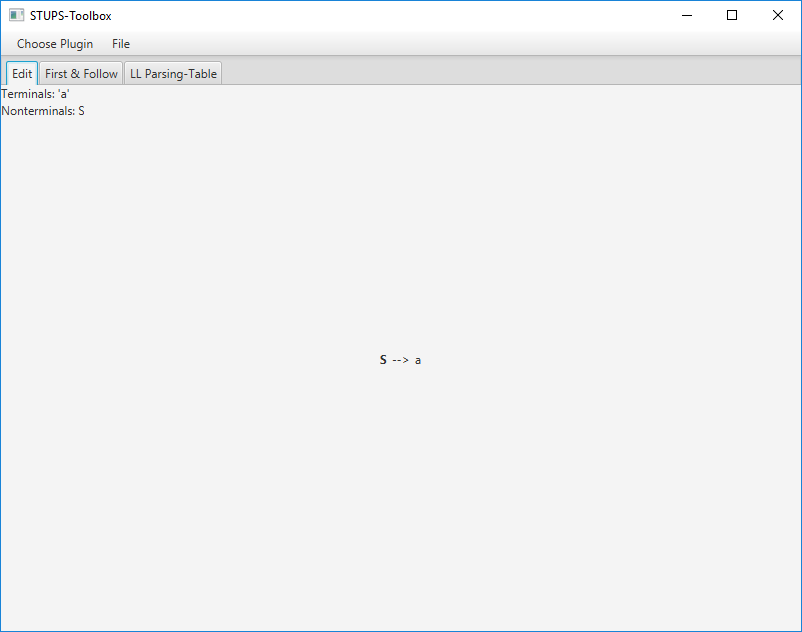
\includegraphics[width=1\textwidth]{bilder/gui_alt.png}
	\caption{Die GUI der Toolbox 1.0}
	\label{img:oldgui}
\end{figure}


\lstset{
	language=Java,
	breaklines=true,
	commentstyle=\color{orange},
	keywordstyle=\color{blue},
	stringstyle=\color{purple},
	rulecolor=\color{black}
}
\section{Benutzerebene}\raggedbottom
Viele der �nderung betreffen die Funktionalit�t der Toolbox und sind f�r den Benutzer direkt ersichtlich. Im Folgenden wird auf diese �nderungen auf Nutzerebene eingegangen. 
\subsection{GUI-Design}
Die Benutzeroberfl�che (\textit{GUI}) ist modernisiert worden. Sie hat bunte Elemente erhalten, die sich per css-Stylesheet anpassen lassen.
Au�erdem wurde vesucht, die Bedienung intuitiver zu gestalten.
Eine Abbildung der GUI findet sich in Abb. \ref{img:gui}. 
\paragraph{Aufbau}
Beim Design der GUI wurde sich an bekannten IDEs, wie zum Beispiel IntelliJ
Idea\footnote{\url{https://www.jetbrains.com/idea/}}, orientiert.
Im linken Teil der GUI befindet sich ein Baum mit drei Unterknoten: Grammar,
PushDownAutomaton (Kellerautomat) und Automaton.
Klappt man diese Unterknoten auf, erh�lt man eine �bersicht �ber alle momentan
gespeicherten Objekte dieses Types.
Eine Abbildung der GUI findet sich in Abb. \ref{img:gui}. 
\paragraph{Bedienung}
�ber den Baum lassen sich die verschiedenen Objekte ausw�hlen und werden im rechten Teil
dargestellt.
Im unteren rechten Teil befinden sich die ComplexFunctionPlugins. Diese arbeiten immer auf dem aktuell ausgew�hlten Typ
und sind �ber Tabs ausw�hlbar.

Die SimpleFunctionPlugins lassen sich durch Rechtsklick auf das Objekt im Baum, auf
dem sie durchgef�hrt werden sollen, aufrufen.
Es gibt nun SimpleFunctionPlugins, die auf allen Objekten im Baum arbeiten. Hierzu geh�ren \textit{Print}, \textit{Rename} und \textit{Undo}, welches eine �nderung r�ckg�ngig macht. 
\paragraph{Vorteile}
Die Bedienung ist intuitiver geworden und erm�glicht es, schnell zwischen den 
verschiedenen Datentypen zu wechseln, ohne bestehende �nderungen zu verlieren.
Auch zwischen Objekten desselben Datentypes kann leicht gewechselt werden und 
diese sind dadurch gut vergleichbar.
Die Funktion, eine �nderung r�ckg�ngig zu machen, erm�glicht es, Algorithmen auszuprobieren
und danach die urspr�nglichen Daten ohne viel Aufwand wieder herzustellen.

Alle vorgenommen Einstellungen, wie css-Stylesheets 
oder das Symbol f�r das leere Wort, werden gespeichert, so dass eine komfortable, pers�nliche Modifizierung m�glich ist.
\begin{figure}[htbp]
	\centering
	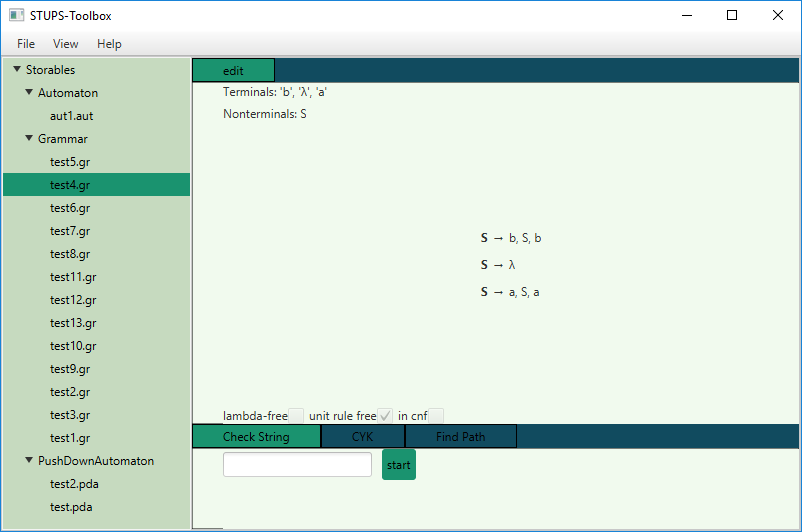
\includegraphics[width=1\textwidth]{bilder/gui.png}
	\caption{Die GUI der Toolbox 2.0}
	\label{img:gui}
\end{figure}


\subsection{Feature-�bersicht}
Im Folgenden werden die neuen Features kurz erkl�rt. Hierbei geht es haupts�chlich um die Ausf�hrung der Befehle, eine genaue Erkl�rung der Algorithmen findet sich in Kapitel \ref{sec:theorie}.

\subsubsection{Ausgabe}
Damit die Durchf�hrung der Algorithmen transparent ist, ist eine dokumentierte Ausf�hrung m�glich. Hierbei wurden die Algorithmen in Schritte eingeteilt, die sich an den Schritten der Algorithmen in \cite{Rot16} orientieren. Auf Wunsch ist eine Ausgabe dieser Dokumentation m�glich.\hfill \\
An dieser Stelle sei bemerkt, dass es in der vorgebebenen Zeit nicht m�glich war, f�r alle bereits bestehenden Funktionen einen Ausgabe zu erstellen.


F�r die Ausgabe gibt es den sogenannnten \textit{Printmodus}. Dieser hat drei Zust�nde: \textit{no, console} und \textit{latex}. 
Im Modus \textit{no} erfolgt keine Ausgabe, im Modus \textit{console} erfolgt eine Ausgabe auf die Konsole und im Modus \textit{latex} eine \LaTeX-konforme Ausgabe in eine kompilierbare \LaTeX -Datei.
Printmodus \textit{no} und \textit{console} werden durch den Befehl \textit{print-mode type} aufgerufen.
Die \textit{GUI} befindet sich standardm��ig im Printmodus \textit{no}.

Der Printmodus \textit{Latex} besitzt dabei einige Besonderheiten, auf die im n�chsten Abschnitt genauer eingegangen wird.
\paragraph{\LaTeX}
Kombilierbarer \LaTeX -Code wird nur erzeugt, wenn die Toolbox sich im Printmodus \textit{latex} befindet.Dieser muss manuell gestartet und auch wieder beendet werden.
Der Printmodus \textit{latex} wird �ber das Kommando \textit{print-mode latex path/to/file} (oder in der GUI �ber \textit{Export $\rightarrow$ Latex $\rightarrow$ Start Latex Export}) gestartet. Das Beenden des \LaTeX -Modus geschieht durch den Wechsel in einen anderen \textit{Printmodus}
per Konsolenbefehl \textit{print-mode no} oder \textit{print-mode console}, durch das �ffnen oder Schlie�en der GUI
oder in der GUI �ber  \textit{Export $\rightarrow$ Latex $\rightarrow$ End Latex Export}.

W�hrend das Programm im Printmodus \textit{latex} ist, werden alle durchgef�hrten Befehle mit Ausgabe in die ausgew�hlte Datei geschrieben. 

\subsubsection{Grammatiken}
\paragraph{Entfernen von $\lambda$-Regeln}
$\lambda$-Regeln sind Regeln der Form $A \rightarrow \lambda$. $\lambda$-Regeln lassen sich per SimpleFunctionPlugin \textit{Remove $\lambda$-Rules} oder per Konsolenbefehl \textit{rlr} entfernen.
\paragraph{Entfernen von einfachen Regeln}
Einfache Regeln (\textit{Unit Rules}) sind Regeln der Form $A \rightarrow B$. Sie lassen sich per SimpleFunctionPlugin \textit{Eliminate Unit Rules} oder per Konsolenbefehl \textit{eur} entfernen.
\paragraph{Chomsky-Normal-Form (CNF)}
Die CNF ist eine Normalform, die nach dem Linguisten Noam Chomsky benannt ist. Eine Grammatik l�sst sich per SimpleFunctionPlugin \textit{CNF} oder per Konsolenbefehl \textit{cnf} in CNF umformen.
\paragraph{CYK-Algorithmus}
Der CYK-Algorithmus l�st in kubischer Zeit das Wortproblem f�r kontextfreie Sprachen. Der CYK-Algorithmus wurde �ber ein ComplexFunctionPlugin implementiert. Hierzu muss im Bereich der ComplexFunctionPlugin der Tab ``CYK''' ausgew�hlt und in dem Textfeld das zu untersuchende Wort eingegeben werden. Zu Beachten ist, dass die einzelnen Buchstaben durch Leerzeichen getrennt werden m�ssen. Der Button ``Go''' startet den Algorithmus.
\paragraph{Vereinfachung}
Per SimpleFunctionPlugin l�sst sich eine Grammatik vereinfachen. Hierbei werden Nichtterminale erkannt und entfernt, die redundant, nicht erreichbar oder ohne weiterf�hrende Regeln sind. Falls die Grammatik in Chomsky-Normalform ist, bleibt diese Eigenschaft bestehen.
\paragraph{Umwandlung in Kellerautomat}
Eine Grammatik l�sst sich per SimpleFunctionPlugin \textit{To PDA} oder Konsolenbefehl \textit{topda} in einen Kellerautomaten umwandeln.
\paragraph{Interaktives Ableiten (nur GUI)}
Als ComplexFunctionPlugin wurde die M�glichkeit implementiert, eine interaktive Ableitung zu erstellen. %todo

\subsubsection{Kellerautomaten}
kellerautomaten wurden als neuer Datentyp eingef�hrt, da sie die kontextfreien Grammatiken gut erg�nzen auf Grund der bestehenden �quivalenzbeziehung.
\paragraph{Umwandeln in Grammatik}
Ein Kellerautomat l�sst sich per SimpleFunctionPlugin \textit{To Grammar} oder Konsolenbefehl \textit{togrammar} in eine �quivalente Grammatik umwandeln
\paragraph{ Bearbeitung (nur GUI)} 
Die Regeln eines Kellerautomatens sind durch \textit{Buttons} dargestellt. Durch Rechtsklick oder Doppelklick auf eine Regel, �ffnet sich ein sich zun�chst ein Men�, in dem ausgew�hlt werden kann, ob die Regel bearbeitet oder gel�scht werden soll. W�hlt man Ersteres, �ffner sich ein Dialog zum Bearbeiten.
\paragraph{Schritt-f�r-Schritt Durchlauf (nur GUI)} 
Das ComplexFunctionPlugin ``Check String''' liefert dem Benutzer die M�glichkeit, interaktiv zu pr�fen, ob ein Wort in der Sprache des Automaten liegt. Hierf�r bietet das Plugin ein Textfeld und einen ``Start'''- und ``Undo'''-Button an. In das Textfeld muss das Wort eingegeben werden, auch hier wieder Trennung der Buchstaben durch Leerzeichen. Der Button ``Start''' startet das Plugin. Nun ver�ndern sich die Buttons, die die Regeln des Automatens darstellen. Es sind immer nur die Regel ausw�hlbar, die auch tats�chlich auf den aktuellen Input und \textit{Top of Stack} passen. Durch Klick auf eine Regel wird diese angewandt. Dies kann so lange gemacht werden, bis ein Pfad gefunden wurde, oder keine Regel mehr anwendbar ist.


\subsection{Sonstiges}
\begin{itemize}
\item Der Hilfe-Text (aufrufbar durch den Konsolenbefehl \textit{help}) wurde so formatiert, dass er �bersichtlicher ist.
Hierzu geh�rte das Einr�cken der Beschreibungen und eine Sortierung nach dem Alphabet.
\item Das leere Wort wird nun nicht mehr als Bestandteil der Terminalmenge angezeigt. Auch beim Parser einer Grammatik muss das leere Wort nicht mehr in der Terminalmenge inkludiert werden.
\item "`epsilon"', "`lambda"' und "`->"' wurden in der GUI durch entsprechende ASCII-Zeichen ersetzt.
\item durch "`u"' und "`d"' l�sst sich die Schrift in der GUI vergr��ern bzw. verkleinern.
\item in der GUI gibt es jetzt Tooltips, die die Bedienung erkl�ren. 
\end{itemize}
\section{Build-Prozess}
Als Build-Prozess wird die automatische Erstellung eines fertigen, ausf�hrbaren Programmes bezeichnet.
Bisher wurde dies �ber ein \textit{Makefile} umgesetzt. Dies hatte den Nachteil, dass das Ausf�hren nicht plattformunabh�ngig gewesen ist.
Au�erdem war es unter Anderem auf Grund der externen Bibliotheken nicht m�glich, eine JAR erstellen zu lassen.

Um plattformunabh�ngig zu entwickeln, wurde der Build-Prozess von \textit{Makefiles} auf \textit{Gradle} umgestellt. Gradle\footnote{\url{https://gradle.org/}} ist ein automatisches Build-Tool, welches plattformunabh�ngig ist. Dies erforderte einige Anpassungen des von SableCC erzeugten Codes.
  
  
\subsection{Gradle}\label{Gradle}
Als Build-Tool wurde sich f�r Gradle\footnote{\url{https://gradle.org/}} entschieden. Es ist plattformunabh�ngig und verf�gt �ber die M�glichkeit mit \textit{Groovy}\footnote{\url{http://groovy-lang.org/}}  ausf�hrbare Skripte zu erstellen, was im Folgenden wichtig wird.

F�r die Umstellung musste zun�chst der Aufbau der Packages angepasst werden. Gradle setzt
eine Trennung von Source-Code und Resourcen voraus.
Des Weiteren erwartet Gradle folgende Ordnersturktur: \\

\begin{minipage}[htbp]{\linewidth}
\begin{description}
\item[src]\hfill 
	\begin{description}
	\item[main] \hfill 
		\begin{description}
		\item[java] 
		\item[resource]
		\end{description}
	\item[test] \hfill 
		\begin{description}
			\item[java]
			\item[resource]
			\end{description}
		\end{description}
\end{description}
\end{minipage}\\

Es wurde au�erdem ein weiterer Source-Ordner \textit{GeneratedSource} angelegt, der
die von Gradle generierten Dateien enth�lt.
Gradle sorgt daf�r, dass alle ben�tigten Bibiliotheken heruntergeladen werden
und zum \textit{Java-Classpath} hinzugef�gt werden.
Durch ein Plugin\footnote{\url{https://github.com/johnrengelman/shadow}} kann eine ausf�hrbare .jar-Datei
erzeugt werden, die die importierten Bibliotheken enth�lt. Dies war vorher
nicht m�glich.

\subsubsection{Gradle und SableCC}
Das Zusammenspiel von Gradle und SableCC gestaltete sich nicht einfach. SableCC
ist ein Parser-Generator, welcher von Etienne M. Gagnon entwickelt
wurde\footnote{\url{http://www.sablecc.org/}}. Durch SableCC werden Java-Dateien und Resourcen erzeugt. Leider vermischt SableCC diese.
 Dies hat zur Folge, dass diese Resourcen nicht mehr gefunden werden, da
auf diese mit \textit{getResource} zugegriffen wird und sie sich nicht im
Resource-Ordner befinden, wo Java die Dateien nach Umstellung auf Gradle sucht.

Es war also n�tig, Groovy-Code \ref{lst:build} zu
schreiben, welcher nach dem Build-Prozess die ben�tigten Resourcen in Unterordner des Resource Ordner
von \textit{GeneratedSources} kopiert und anschlie�end die entsprechende
\textit{getResource} Zeilen auf diesen Unterordner anpasst.

\begin{figure}[htb]
\lstinputlisting[frame=single, basicstyle=\small, label=lst:build, caption=Gradle-SableCC-Workaround]{Code/build.gradle}
\end{figure}

Die Toolbox besitzt dabei folgenden Abh�ngigkeiten:
\begin{description}
	\item[JUNG2]\footnote{\url{http://jung.sourceforge.net/}}  Zur Darstellung von Automaten
	\item[JUnit 4]\footnote{\url{http://junit.org/junit4/}} Zum Testen von Code
	\item[Apache Commons-IO]\footnote{\url{http://commons.apache.org/proper/commons-io/}} Zum Bearbeiten von Ordner (wird f�r den Workspace gebraucht)
	\item[Reflections]\footnote{\url{https://github.com/ronmamo/reflections}} Erstellen von Objekten zur Laufzeit, auch in der .jar
	\item[SableCC]\footnote{\url{http://www.sablecc.org/}} Parser-Generator
	\item[Apache Commons Lang]\footnote{\url{https://commons.apache.org/proper/commons-lang/}}  Zum �berschreiben der \textit{equals} und \textit{hashCode}-Methoden
\end{description}

\subsubsection{Build}
Folgende Befehle sind durch die bereitgestellte ausf�hrbare Gradle-Datei aufrufbar:
\begin{itemize}
\item gradle shadowJar \hfill \\
Erstellt eine ausf�hrbare Jar in build/libs.
\item gradle sableCC \hfill \\
Startet SableCC und erstellt die notwendigen Parser. Dieser Befehl ist in dem Befehl \textit{build} enthalten.
\item gradle javadoc \hfill \\
Erstellt die Dokumentation.
\item gradle eclipse \hfill \\
Erm�glicht es, das Programm als Eclipse Projekt zu importieren
\item gradle idea \hfill \\
Erm�glicht es, das Programm als IntelliJ Projekt zu importieren
\item gradle build \hfill \\
Ein kompletter Build.
\end{itemize}

\section{Entwicklung}\raggedbottom
Wie schon am Anfang erw�hnt, ist dies ein fortgef�hrtes Projekt. Die Weiterentwicklung eines bereits bestehenden Programmes bietet andere Herausforderungen als 
die alleinige Entwicklung. Einige Aspekte des Programmes waren nicht mit den Anforderungen dieser Arbeit kompatibel und mussten ge�ndert werden. Im Folgenden wird auf einige notwendige �nderungen und Verbesserungen eingegangen

\subsection{Aufbau der Toolbox}
Der Aufbau der Packages war nicht optimal. Wie oben erw�hnt, ben�tigt Gradle eine strikte Trennung von Source und Resource. Dies wurde durch Anpassung der Packages erreicht. Au�erdem war es n�tig, \textit{CLI} und \textit{GUI} aus dem Wurzelverzeichnis in ein eigenes Package zu verschieben, sodass diese Klasse von anderen importiert werden k�nnen. Im Folgenden wird kurz auf die einzelnen Packages und ihre Aufgaben eingegangen.
\begin{description}
\item[Automaton Simulator]
Dieses Package beeinhaltet die Modelle, die ben�tigt werden, um Automaten
darzustellen. Die Logik befindet sich in der Klasse \textit{AutomatonUtil}.
Die Klasse \textit{Visitor} stellt die Schnittstelle zu SableCC her und ist f�r das Parsen von
Automaten aus Dateien zust�ndig.
\item[Grammar Simulator]
Dieses Package beinhaltet die Modelle, die ben�tigt werden, Grammatiken
darzustellen und Algorithmen auf diesen duchrzuf�hren. Genau wie bei den
Automaten stellt \textit{Visitor} die Verbindung zu SableCC her und \textit{GrammarUtil} beinhaltet die Logik.
\item[PushDownSimulator]
Dieses Package beinhaltet die Modelle f�r Kellerautomaten (Pushdown Automatons).
\textit{PushDownAutomatonUtil} enth�lt Funktionen f�r Kellerautomaten und \textit{Visitor}
ist f�r das Parsen von Kellerautomaten aus Dateien zust�ndig.
\item[CLIPlugins]
In diesem Package finden sich die Kommandozeilenprogramme. Jedes der Plugins
muss die abstrakte Klasse \textit{CLIPlugin} erweitern, damit es automatisch
eingebunden wird. Genaueres dazu findet sich in \cite{Ruh16}.
\item[GUIPlugins] \hfill
	\begin{description}
	\item[ComplexFunctionPlugins]
	Hier finden sich GUIPlugins, die eine Benutzereingabe ben�tigen. 
	\item[DisplayPlugins]
	Die Klassen in diesem Package sind f�r die Darstellung der Modelle zust�ndig.
	\item[SimpleFunctionplugins]
	SimpleFunctionPlugins operieren auf einem Objekt und ben�tigen keine weitere
	Nutzereingabe
	\end{description}
\item[Main]
Das Package \textit{Main} beinhaltet unter Anderem die Klassen \textit{CLI} und \textit{GUI}, welche
vorher im Wurzelverzeichnis waren. Diese beiden Klassen sind das Herzst�ck des
Programmes.
Au�erdem findet sich in dem Package die Klasse \textit{StateController}, die daf�r
sorgt, dass sich das Programm nach Neustart im selben Zustand befindet wie es beendet wurde, und die Klasse \textit{Content}, die die gespeicherten Objekte
enth�lt und verwaltet.
Durch diese beiden neuen Klassen wurde versucht, eine gr��ere Aufgabentrennung zu
erreichen. 
\item[Print]
In diesem Package ist die Hauptklasse die Klassen \textit{Printer}, die f�r jegliche
Art von Schreiboperationen zust�ndig ist.
Die Enumeration \textit{Printmode} enth�lt die Typen \textit{NO}, f�r kein Drucken,
\textit{CONSOLE} f�r Ausgabe auf das Terminal und \textit{LATEX} f�r die Ausgabe in eine
\LaTeX-Datei.
\end{description}

\subsection{Umgang mit Objekten}
Vor der Arbeit bestand der Wunsch, die vollf�hrten �nderungen r�ckg�ngig machen
zu k�nnen. Hierzu ist es n�tig, dass Objekt in seinem \textit{Vorher-Zustand} zu
speichern. Leider hatte die Toolbox 1.0 diese M�glichkeit nicht, da jeder
Algorithmus auf dem selben Objekt arbeitete und dieses ver�nderte. Es war also
nicht (einfach) m�glich, eine \textit{Vorher-Version} zu speichern.

Um dies zu �ndern, wurde zun�chst eine Methode eingef�hrt, die eine
\textit{deep-copy} des Objektes anlegt, also ein Objekt, welches die gleichen
Eigenschaften, aber nicht die selben Referenzen hat.
Der Nachteil hieran war, dass vor jeder �nderung manuell eine fr�here Version
gespeichert werden musste.
Daher wurden im n�chsten Schritt die Objekte `\textit{immutable}
gemacht.\footnote{Link}, d.h. die Objekte sind nach ihrer Erstellen %todo% besseres Wort
nicht mehr ver�nderbar. Der Programmierer wird gezwungen, f�r jede �nderung ein
neues Objekt anzulegen. Dies erscheint auf den ersten Blick unpraktisch, stellte
sich jedoch als keine gro�e Unannehmlichkeit heraus.
Diese Ver�nderung liefert direkt mehrere Vorteile: 


\begin{minipage}{\textwidth}
\begin{itemize}
  \item eine Objektreferenz auf die Vorg�ngerversion muss direkt im Konstruktor
  bestimmt werden
  \item beim Ver�ndern der Regelmenge einer Grammatik oder eines
  Kellerautomaten ist es nun nicht mehr n�tig, die Menge der Terminale und
  Nichtterminale anzupassen, da diese automatisch im Konstruktor aus der Regelmenge bestimmt werden
  \item es kommt zu keinen Konflikten mehr mit der Hashcode-Berechnung.
  Ver�ndert sich ein Objekt, so ver�ndert sich auch sein Hashcode. Daher sollten Objekte
  in HashSets nicht mehr ver�ndert werden. Dies war in der alten Toolbox nicht
  gew�hrleistet
\end{itemize}
\end{minipage} \\

Es war nicht nur n�tig, die Variablen der Klasse mit dem Kennwort \textit{final} zu kennzeichnen und die Setter-Methoden zu entfernen, es musste auch daf�r gesorgt werden, dass bestehenden Listen oder Sets keine Elemente hinzugef�gt oder gel�scht werden. Hierf�r wurde in den Getter-Methoden mithilfe von \textit{Collections.unmodifiableSet} bzw \textit{Collections.unmodifiableList}\footnote{\url{https://docs.oracle.com/javase/7/docs/api/java/util/Collections.html}} unmodifizierbare Mengen bzw. Listen zur�ckgegeben.


Aufgrund der recht komplexen, bestehenden Algorithmen auf Automaten, die h�ufig
auf die Setter-Methoden zugreifen, war es nicht m�glich in der gegebenen Zeit, die Automaten
unmodifizierbar zu machen. Daher wird weiterhin bei Automaten mit der
\textit{deep-copy}-Methode gearbeitet.


Als weiteres Feature ist nun das parallele Arbeiten mit mehren Objekten eines
Types m�glich. Dazu wurde ein sogenannter \textit{Store} eingef�hrt, der die Objekte
f�r den Nutzer aufbewahrt und verwaltet. Die Objekte, die im Store gespeichert
werden, m�ssen das Interface \textit{Storable} implementieren.

\begin{minipage}{\textwidth}
\lstinputlisting[frame=single, basicstyle=\small, caption=Das Interface
\textit{Storable}]{Code/Storable.java}
\end{minipage} 

Durch das Plugin wird gew�hrleistet, dass jede Klasse eine
\textit{deep-copy}-Methode hat. Bei Grammar und PushDownAutomaten wird hier
einfach ein neues Objekt erstellt. Dieses ist automatisch wegen der
Unmodifizierbarkeit eine echte Kopie.
Die Methoden \textit{printToSave} und \textit{restoreFromFile} k�mmern sich um das Laden und Speichern des Objektes.
Wie im vorherigen Abschnitt erkl�rt, liefert die Methode \textit{getPreviousVersion} die Vorg�ngerversion des Objektes.
\textit{printLatex} und \textit{printConsole} sind Methoden aus dem Interface Printable und werden genauer in Abschnitt \ref{sec:Printer} erkl�rt.

Das Interface hat auch den gro�en Vorteil, dass Grammar, PushDownAutomaten,
Automaten, \ldots einen gemeinsamen Typ haben. Au�erdem fiel bei vielen Funktionen die Fallunterscheidung weg, da eine generische Ausf�hrung m�glich geworden ist.

Beim Laden eines Objektes in der Konsole muss es
zun�chst manuell im Store gespeichert werden. Es gibt weiterhin genau
ein aktuelles Objekt jeden Types, der Nutzer kann diese jedoch mit dem Befehl \textit{switch type name}
(bzw in der GUI durch den Baum) �ndern. Die Plugin operieren immer noch auf
diesem aktuellen Element.

Im Zuge dieser �nderungen wurde gleichzeitig die Vergleichbarkeit von Komponenten von Grammatiken, Automaten und
Kellerautomaten erm�glicht.
Hierf�r wurden die \textit{equals}- und \textit{hashCode}-Methode mit Hilfe der Bibliothek Apache Commons-lang\footnote{\url{https://commons.apache.org/proper/commons-lang/}} �berschrieben. Das �berschreiben der \textit{hashCode}-Methode ist wichtig, da es sonst zu Unregelm��igkeiten im Verhalten von \textit{HashSets} kommt.

Bei einigen Objekten war dies technisch jedoch zun�chst gar nicht m�glich.
So zum Beispiel bei Nichtterminalen, die Referenzen auf die Regeln,
bei denen sie auf der linken Seite stehen, enthielten. Dadurch gab es zyklische Referenzen und ein sinnvolles �berschreiben der \textit{equals}-Methode war nicht m�glich. Daher wurde die Klasse \textit{Rule} eingef�hrt, die eine Produktionsregel einer Grammatik beschreibt und die Grammatik selbst enth�lt jetzt ein \textit{Set} mit allen ihren Regeln. Die Nichtterminale selbst enthalten keine Regeln mehr.
Hierdurch ist der Vergleicht von zwei Nichtterminalen sehr einfach geworden. Sie sind genau dann gleich, wenn sie den 
gleichen Namen haben.

Diese Vergleichbarkeit erleichterte die Durchf�hrung vieler Algorithmen, da es nicht mehr wichtig war, genau die richtige Referenz zu haben.
Hierzu ein kleines Beispiel:

Wollte man eine neue Regel $A \rightarrow a, B, C$, mit $A,B,C$ Nichtterminal und $a$ Terminal, zu einer Grammatik hinzuf�gen, musste man zun�chst aus der Menge der Nichtterminale das Objekt suchen, dass den gew�nschten Namen "`A"' hat. Nun muss jedes Element auf der rechten Seite in der Menge der Terminale und Nichtterminal gesucht und genau dieses Objekt einer Liste hinzugef�gt werden.
Diese Liste wird dann dann der Regelmenge von Nichtterminal "`A"' hinzugef�gt.

\begin{minipage}{\textwidth}
\begin{lstlisting}[frame=single,caption={Das Erstellen einer Regel},label=lst:rule]
public Grammar addRule(Grammar g) {
	List<Symbol> tmp = new ArrayList<>();
	tmp.add(new Terminal("a"));
	tmp.add(new Nonterminal("B"));
	tmp.add(new Nonterminal("C"));
	Rule rule = new Rule(new Nonterminal("A"),tmp)
	Set<Rule> rules = new HashSet<Rule>(grammar.getRules());
	rules.add(rule);
	return new Grammar(grammar.getStartsymbol,rules,grammar.getName(),grammar);
}
\end{lstlisting}
\end{minipage}

Mit den �nderung ist dies viel einfacher geworden. Mit dem Code in \ref{lst:rule} wird eine neue Regel erstellt und der Grammatik hinzugef�gt.
Wie man sieht, ist es nicht n�tig, die Referenz der Symbole herausfinden; man kann einfach neue Objekte erstellen.\\

Hier wird nochmal die Unmodifizierbarkeit deutlich. Es ist nicht m�glich, die Regel direkt der Menge der Regeln hinzuzuf�gen. Stattdessen wird eine tempor�re Regelmenge
erstellt und dann eine neue Grammatik, die diese neue Regelmenge hat.

\subsection{Persistierung der Objekte}
Wie man im vorherigen Abschnitt gesehen hat, stellt das Interface \textit{Storable}
Methoden zum Speichern und Laden zur Verf�gung. Beim Beenden des Programmes
werden die vollf�hrten �nderung automatisch gespeichert und beim n�chsten Start
wieder geladen.

Das Programm \textit{merkt} sich �nderungen in einer \textit{config}-Datei.
Die \textit{config}-Datei sorgt daf�r, dass das Programm im selben Zustand
startet, wie es beendet wurde.
In ihr wird unter Anderem der Ordner des aktuellen Workspaces, der Name des
Nullsymbols, dass der User ausgew�hlt hat und das aktuelle css-Stylesheet
gespeichert. Den Aufbau der \textit{config}-Datei sieht man in \ref{config}.

\begin{minipage}{\textwidth}
\lstinputlisting[frame=single, basicstyle=\small, caption=Die
\textit{Config}-Datei,label=config]{Code/config.config} 
\end{minipage}

Um einen zentralen Ort f�r die Speicherung der Objekte zu haben, wurde ein sogenannter \textit{Workspace} eingef�hrt. Auch hier wurde sich wieder an einer IDE orientiert.
Alle Dateien des Workspaces sind in der GUI im Baum sichtbar. Der Workspace hat ein Pendant auf der
Festplatte. Standardm��ig ist dies der Ordner \textit{workspace} im Verzeichnis des Programms.
Auf Wunsch kann der Workspace, momentan nur in der GUI, gewechselt werden. 

Um eine problemlose Persistierung zu erm�glichen, wird bereits in der GUI verhindert,
dass ung�ltige Namen f�r Terminale und Nichtterminale eingegeben werden.
Hierzu geh�ren bei Terminalen der Gebrauch von des Hochkomma \grq{} und bei Nichtterminalen alles au�er Buchstaben, Zahlen und \_.

\subsection{Kellerautomaten}
Kellerautomaten (PDA) wurden als neuer Datentyp implementiert. Ein Kellerautomat
besteht aus einer Menge von Zust�nden (states), einem Eingabe-Alphabet
(inputAlphabet), einem Stack-Alphabet (stackAlphabet), einem Startzustand
(startState), einem Bottom-Symbol f�r den Stack (initialStackLetter), einer
Menge von Produktionsregeln (rules) und dem aktuellen Zustand, in dem sich der
PDA befindet (currentState). Ein PDA akzeptiert in dieser Implementierung ein
Wort, wenn der Stack leer ist.\\
Die Darstellung der Klasse in \ref{lst:pda} ist stark verk�rzt, um nur die wichtigsten Aspekte zu zeigen.

Wie man sieht, ist es nicht n�tig, dem PDA Zust�nde, Input- und Stack-Alphabet zu �bergeben, da 
diese im Konstruktor bestimmt werden. Dies ist nur dank der Unmodifizierbarkeit m�glich, da sich die genannten Mengen
nach Erstellung des Objekts nicht mehr ver�ndern.

\begin{minipage}{\textwidth}
\noindent
\lstinputlisting[frame=single, basicstyle=\small, label=lst:pda, caption=Die Klasse
\textit{Pushdownautomaton}]{Code/PushDownAutomaton.java}
\end{minipage}


 Die Unmodifizierbarkeit wird auch bei der Betrachtung der Getter- und Setter-Methoden deutlich: \hfill \\
Aufgrund der fehlenden Setter-Methoden ist es nicht m�glich, einzelne Werte zu ver�ndern.
Auch das Hinzuf�gen in \textit{List} und \textit{Set} wurde durch den
Aufruf von
\textit{Collections.unmodifiableList} bzw. \textit{Collections.unmodifiableSet}
in den Getter-Methoden verhindert.

\subsection{Ausf�hrbare JAR}

\begin{figure}[htbp]\label{reflections}
	\begin{minipage}[t]{0.45\textwidth}
\begin{lstlisting}[frame=single, basicstyle=\tiny, caption={ Toolbox 1.0}]
 try {
  String packagePath = Thread.currentThread()
    .getContextClassLoader()
    .getResources("CLIPlugins")
    .nextElement().getFile().replace("%20", " ");
  File[] classes = new File(packagePath).listFiles();
  URLClassLoader urlClassLoader = URLClassLoader
    .newInstance(new URL[]{new URL("file://" + packagePath)});
  for(File file : classes) {
    if(file.getName().endsWith(".class") 
       && !file.getName().equals("CLIPlugin.class") 
       && !file.getName().contains("$")) {
        plugins.add((CLIPlugin) urlClassLoader
        .loadClass("CLIPlugins." + file.getName()
        .substring(0, file.getName().length() - 6))
        .newInstance());
    }
  }
} catch(Exception e) {
 e.printStackTrace();
}
\end{lstlisting}
	\end{minipage}
\hfill
	\begin{minipage}[t]{0.45\textwidth} 
\begin{lstlisting}[frame=single, basicstyle=\tiny, caption={Toolbox 2.0}]
Reflections refl=new Reflections("CLIPlugins");
Set<Class<? extends CLIPlugin>> s=refl.
	getSubTypesOf(CLIPlugin.class);
s.forEach(r -> {
  try {
    CLIPlugin plugin = r.newInstance();
     plugins.add(plugin);
  } catch (InstantiationException | IllegalAccessException e) {
    e.printStackTrace();
  }
});
	\end{lstlisting}
	\end{minipage}
\end{figure}
Es war bei der Toolbox 1.0 unter Anderem wegen der Erzeugung von Objekten zur Laufzeit mit Hilfe des \textit{URLClassLoaders}\footnote{Link} nicht m�glich, eine ausf�hrbare JAR zu erzeugen.
Dies ist durch die Verwendung von Reflections und die im Abschnitt \ref{Gradle} erw�hnten �nderungen m�glich geworden.

Der Codeausschnitte \ref{reflections} aus der Klasse \textit{CLI} zeigt beispielsweise die
Ver�nderung beim Laden der CLI-Plugins. 
Der Code erm�glicht nicht nur die Ausf�hrugn als JAR, er ist auch k�rzer und �bersichtlicher

\subsection{Ausgabe} \label{sec:Printer}

Die bisherige Toolbox besa� eine Ausgabe auf die Konsole. Diese war starr geregelt und daher nicht erweiterbar. Da aber nun auch eine Ausgabe in .tex-Datein m�glich sein sollte, musste die Ausgabe �berarbeitet werden, und zwar so, dass in Zukunft auch andere Ausgabe-Modi (html, xml) leicht hinzu programmiert werden k�nnen.
Dazu wurde die Ausgabe zun�chst gekapselt an das Package \textit{Print} abgegeben, welches f�r die richtige Ausgabe sorgt. 
\subsubsection{Das Interface \textit{Printable}}
Wenn man ein Objekt drucken m�chte, soll man sich keine Gedanken dar�ber machen, in welcher Form das geschieht. Man m�chte die Ausgabe nicht selber formatieren. Es w�re w�nschenswert, wenn das Objekt selbst wei�, wie es zu drucken ist. Daher wurde das Interface \textit{Printable} eingef�hrt. Dieses stellt zwei Methoden zur Verf�gung: \textit{printConsole}, welches f�r die Ausgabe auf die Konsole zust�ndig ist, und \textit{printLatex}, welches f�r die \LaTeX-konforme Ausgabe sorgt.

Das Interface \textit{Storable} erweitert \textit{Printable}, da alle speicherbaren Objekte auch druckbar seien sollen. 

\subsubsection{Die Klasse \textit{Printer}}
Die \textit{Printer}-Klasse ist f�r die Ausgabe von Objekten und Umformungen zust�ndig und stellt einen wichtigen Teil des Programmes dar.
In diesem Abschnitt werden kurz die wichtigsten Funktionen erl�utert.

\begin{minipage}{\linewidth}
\begin{lstlisting}[frame=single,caption={Die Klasse \textit{Printer}},label=lst:print]
public class Printer {
    private static PrintMode printmode=PrintMode.CONSOLE;
    private static BufferedWriter writer=new BufferedWriter(new OutputStreamWriter(System.out));
    public static void print(Printable printable) {
        switch (printmode) {
            case NO:
                break;
            case LATEX:
                printable.printLatex(getSpace(deepness));
                break;
            case CONSOLE:
                printable.printConsole();
                break;
        }
    }
    public static void printEnumeration(ArrayList<Printable> printables, String[] pointdescriptions, String[] texts, String title) {
        switch(printmode) {
            case NO:
                break;
            case CONSOLE:
                printEnumerationConsole(printables,pointdescriptions,texts);
                break;
            case LATEX:
                printEnumerationLatex(printables,toLatex(pointdescriptions),toLatex(texts),toLatex(title));
                break;
        }
    }
   //...
}
\end{lstlisting}
\end{minipage}

Listing \ref{lst:print} stellt die zentralen Komponenten der Klasse dar. Die Klasse \textit{Printer} besitzt ein \textit{PrintMode printmode}, dies gibt an,
in welchem Printmodus der Printer sich momentan befindet.
Dazu gibt es einen \textit{BufferedWriter writer}, der passend initialisiert wird. Idealerweise sollte der writer auf die Konsole schreiben, wenn der Printmodus
\textit{CONSOLE} ist und in eine Datei, wenn der Printmodus \textit{LATEX} ist.
Dies ist jedoch nicht festgelegt, sodass beispielsweise die M�glichkeit besteht, Konsolenausgabe in eine Datei zu schreiben.

Die Methode \textit{print(Printable printable)} sollte zum Schreiben von \textit{printable} Objekten genutzt werden. Anhand des printmodes wird entschieden, welche der Methoden \textit{printConsole()} und \textit{printLatex(String space)} des Printables aufgerufen werden soll.
Diese Art der Ausgabe ist vor dem direkten Aufruf von  \textit{printConsole()} und \textit{printLatex(String space)} zu bevorzugen, da so die Verantwortung des richtigen Druckens an den Printer abgegeben wird.



Eine weitere Methode ist  \textit{printEnumeration}. Dies gibt eine Aufz�hlung aus. Auch hier gibt es wieder eine Version f�r die Konsole und eine f�r Latex. 
Es soll eine Aufz�hlung geschrieben werden, deren einzelne Punkte die �berschriften in \textit{pointdescriptions} haben. Dann folgt die Ausgabe eines beschreibenden Textes aus dem dritten Argument \textit{texts} und die Ausgabe eines Elementes aus dem ersten Argument \textit{printables}. Der Titel der Aufz�hlung ist \textit{title}.

\subsection{Generierung \LaTeX}\label{latex}
Ein weitere Funktion der Toolbox ist das Generieren von \LaTeX -Code, welcher die
vom Nutzer durchgef�hrten Schritte darstellt.

Wichtig hierbei war, darauf zu achten, dass \LaTeX-Sonderzeichen erkannt und angepasst werden, damit die entstandene \LaTeX-Datei kompilierbar ist.

Die \LaTeX -Generierung ist nicht automatisch aktiviert. Der Nutzer muss den
\textit{\LaTeX}-Modus starten.
Durch Starten des \LaTeX - Modus wird die Pr�ambel \ref{pre} geschrieben.


\begin{figure}[htbp]
\lstinputlisting[frame=single, basicstyle=\small, caption=Die Pr�ambel, language=TeX, label=pre]{Code/Praeambel.tex}
\end{figure}
Die Datei muss nun noch beendet werden. Dies geschieht wieder nicht automatisch
nach Beendigung eines Befehls, sondern es wurde sich bewusst daf�r entschieden,
dass der Nutzer den \LaTeX -Modus manuell beenden
muss. Hierdurch ist es m�glich, mehrere Algorithmen oder Objekte in eine Datei
zu schreiben.

Erst das Beenden des \LaTeX-Modus beendet die Datei mit \ref{lst:ende} und schlie�t den BufferedWriter.

\lstinputlisting[frame=single, basicstyle=\small, caption={Ende \LaTeX}, language=TeX, label=lst:ende]{Code/Ende.tex}


Ein Herausforderung stellte die Ausgabe von Automaten dar. Die Automaten sollten m�glichst automatisch so dargestellt werden, 
dass sie gut und �bersichtlich aussehen und nicht mehr viel nachtr�gliche Verbesserung n�tig ist. \hfill \\
Zur Darstellung der Automaten wird das Paket TikZ\footnote{hier Link} genutzt. Die Zust�nde sind Knoten und die �berg�nge beschriftete Kanten. TikZ erwartet zuerst eine Aufz�hlung aller Knoten.
Die Positionen werden relativ zueinander angegeben. Um ein gutes Ergebnis zu erhalten, werden die Zust�nde von der Toolbox alphanumerisch sortiert,
da dies h�ufig eine sinnvolle Reihenfolge ist.

Dann m�ssen die Kanten angegeben werden.
Hierbei gibt es f�r Kanten von einem Knoten zu sich selbst, die Option \textit{loop below} oder \textit{loop above}. Es wurde sich f�r \textit{loop below} entschieden.
Bei Kanten, die von einem Zustand zu einem anderen Zustand gehen, muss eine Richtung, in die sich die Kante beugt, angegeben werden und ein Winkel.
Als Richtung wurde \textit{bend left} gew�hlt. Dies bewirkt, dass "'Vorw�rtskanten"', also Kanten, die zu einem Knoten weiter hinten in der Aufz�hlung gehen, �ber den Knoten sind und "'R�ckw�rtskanten"' unterhalb.
Die Winkel werden mit Hilfe der L�nge der Kante $length$ und der maximalen L�nge $maxLength$ berechnet.
Hierbei gibt es zwei F�lle:
\begin{enumerate}
\item $maxLength=1$. Der Winkel jeder Kante wird auf $45^\circ$ gesetzt
\item $maxLength>1$. Der Winkel einer Kante wird auf 
	\[ length * 90/maxLength^\circ \]
gesetzt. Dies bewirkt eine gleichm��ige F�cherung auf dem Winkelintervall $[90/maxLength,90]$.
\end{enumerate}

\begin{figure}[hptb]
	% minipage mit (Blind-)Text
	\begin{minipage}[b]{0.48\textwidth} 
	\lstinputlisting[frame=single, basicstyle=\tiny, language=TeX, nolol]{Code/automat.tex}
	\caption{\LaTeX -Code f�r Automaten}
	\end{minipage}
	% Auff�llen des Zwischenraums
	\hfill
	% minipage mit Grafik
	\begin{minipage}[b]{0.48\textwidth}
	
	\begin{tikzpicture}[shorten >=1pt,on grid,node distance=1.5cm,auto]

  \node[state,initial]   (z0)    {z0};
  \node[state]   (z1)  [right of=z0]    {z1};
  \node[state]   (z2)  [right of=z1]    {z2};
  \node[state,accepting]   (z3)  [right of=z2]    {z3};
\path[->]
(z0)    edge [bend left=60] node {b}  (z2)
        edge [bend left=90] node {b}  (z3)
        edge [bend left=30] node {a}  (z1)
(z1)    edge [bend left=30] node {b}  (z2)
        edge [bend left=60] node {c}  (z3)
(z2)    edge [bend left=30] node {b}  (z3)
        edge [bend left=60] node {b}  (z0)
(z3)    edge [loop below]   node {d}  (z3)
        edge [bend left=60] node {a}  (z1)
;
\end{tikzpicture}
	\caption{Ergebnis}
	\end{minipage}
\label{abb:autbspl}
\end{figure}

\subsection{Testen}
Das Testen beanspruchte einen gro�en Teil der Arbeitszeit, da das Testen
gr��tenteils manuell durchgef�hrt werden musste.
Dies hatte mehrere Gr�nde. Zum Einen ist schwer bis gar nicht m�glich,
rechnerisch zu �berpr�fen, ob zwei Grammatiken �quivalent sind.
Die Umformungen, wie z.B. Entfernen von einfachen Regeln, Entfernen von
$\lambda$-Regeln, mussten manuell auf ihre Korrektheit bzgl. der �quivalenz
�berpr�ft werden.
Zum Anderen erwies sich der \LaTeX -Code als gro�e Fehlerquelle. Es mussten alle
Eventualit�ten bedacht werden, so dass keine Zeichen geschrieben werden, mit
denen \LaTeX nicht umgehen kann. Das reine �berpr�fen des Kompilieren reichte
nicht aus, es musste weiterhin auf die korrekte und �sthetische Schreibweise
geachtet werden.

Jedoch wurden, soweit wie m�glich, JUnit-Test verwendet.
Methoden, die eine Grammatik auf gewisse Eigenschaften, wie keine einfache
Regeln oder $\lambda$ - Freiheit �berpr�fen, konnten getestet werden.
Ebenso, ob Algorithmen, die diese Eigenschaften herbei f�hren sollen, dies auch
tats�chlich tun.

Das Verhalten von \textit{equal} und \textit{toHash} wurde ausf�hrlich per JUnit
getestet.

%%%%%%%%%%%%%%%%%%%%%%%%%%%%%%%%%%%%%%%%%%%%%%%%%%%%%%%%%%%%%%%%%%%%%%%





%%%%%%%%%%%%%%%%%%%%%%%%%%%%%%%%%%%%%%%%%%%%%%%%%%%%%%%%%%%%%%%%%%%%%%%%%%%%%



%%%%%%%%%%%%%%%%%%%%%%%%%%%%%%%%%%%%%%%%%%%%%%%%%%%%%%%%%%%%%%%%%%%%%%%%%%%%%%


%%%%%%%%%%%%%%%%%%%%%%%%%%%%%%%%%%%%%%%%%%%%%%%%%%%%%%%%%%%%%%%%%%%%%%%%%%%%%












%%%%%%%%%%%%%%%%%%%%%%%%%%%%%%%%%%%%%%%%%%%%%%%%%%%%%%%%%%%%%%%%%%%%%%%%%%%%%%%%%%%%%%%%%%%%%%%%%%%%%%%%%%%%%%%


%%%%%%%%%%%%%%%%%%%%%%%%%%%%%%%%%%%%%%%%%%%%%%%%%%%%%%%%%%%%%%%%%%%%%%%%%%%%%%%%%%%%%
\section{Theoretische Aspekte}\raggedbottom \label{sec:theorie}
Beim Umsetzen der Algorithmen in echten Code kam es zu einigen Schwierigkeiten,
da die Algorithmen aus didaktischen Gr�nden so geschrieben sind, dass sie f�r
Menschen leicht umsetzbar sind, jedoch nicht so einfach f�r Computer. Ein
pr�gnantes Beispiel hierf�r ist:\\
Finde alle Kreise und entferne sie.\\
F�r einen Menschen sind die Kreise in einem Graphen leicht ersichtlich, ein
Computer muss erst eine Breitensuche laufen lassen und R�ckw�rtskanten
ermitteln.

Alle Beispiele wurden durch die Toolbox generiert und mit leichten Modifizierungen
�bernommen. Die jetzt als Paragraphen erscheinden �berschriften sind 
eigentlich \textit{Sections}, jedoch w�ren sie dann im Inhaltsverzeichnis dieser Arbeit
aufgetaucht.

Die Algorithmen sind, wenn nicht anders angegeben, dem Skript \cite{Rot16} zur Vorlesung \textit{Einf�hrung in die theoretische Informatik} an der Heinrich-Heine-Universit�t entnommen.

Da angedacht ist, die Toolbox in der Lehre zu verwenden,
wurde darauf geachtet, die tats�chlich Umsetzung dicht an den Algorithmen im
Skript zu belassen und die Durchf�hrung nachvollziehbar zu gestalten.
%%%%%%%%%%%%%%%%%%%%%%%%%%%%%%%%%%%%%%%%%%%%%%%%%%%%%%%%%%
\subsection{Kellerautomaten}

\subsubsection{Einen String �berpr�fen} % todo eher woanders hin?
Durch das \textit{ComplexFunctionPlugin CheckStringPDAPlugin} ist es m�glich, zu �berpr�fen, ob ein PDA ein Wort akzeptiert. Hierf�r wurden die Produktionsregeln in der GUI als Buttons dargestellt. Nach Start des Plugins
ist es m�glich, mit diesen Buttons einen Durchlauf zu simulieren.
Es sind immer nur die Regeln ausw�hlbar, die auch mit dem aktuellen Input und dem \textit{Top of Stack}
kompatibel sind.
Intern wurde der Durchlauf durch eine weitere Klasse \textit{RunThroughInfo} erm�glicht. Diese ist eine Konfiguration
eines Durchlaufs.
Der PushDownAutomat hat als einzige ver�nderbare Variable den aktuellen Zustand in dem er sich befindet.
In der \textit{RunThroughInfo} wird der Stack, der einzulesende Input, der aktuelle Zustand und die vorherige  \textit{RunThroughInfo} gespeichert. %todo
Wird eine Regel vom Nutzer ausgew�hlt, wird diese auf die aktuelle \textit{RunThroughInfo} angewandt und dadurch entsteht eine neue Konfiguration, welche die alte Konfiguration als Vorg�nger hat.

\subsubsection{Umwandeln in Grammatik}
Es ist m�glich, einen Kellerautomaten in eine �quivalente Grammatik umzuformen und umgekehrt (\ref{grammar2pda}).
Daf�r muss der Kellerautomat zun�chst in einen �quivalenten Kellerautomaten, der nur 
Regeln der Form $z_i a_i A_i \rightarrow z_j B_{i_1} B_ {i_2} $ hat, umgewandelt werden.
Eine M�glichkeit, dies zu tun, ist in Algorithmus \ref{alg:2tos} angegeben. 


\begin{algorithm}[htbp]
\caption{Umwandeln}
\label{alg:2tos}
\begin{algorithmic} 
\REQUIRE PDA P mit Regeln $zaA \rightarrow z'B_1B_2 \ldots B_k$ mit $k > 2$ 
\ENSURE PDA ohne Regeln $zaA \rightarrow z'B_1B_2 \ldots B_k$ mit $k > 2$
\FORALL{Regel $zaA \rightarrow z'B_1B_2 \ldots B_k$ mit $k > 2$} 
	\STATE W�hle neue Zust�nde $z_1, z_2, \ldots z_{k-2}$ 
	\STATE Ersetze diese Regel durch die folgenden neuen $\delta$-Regeln:
	\begin{align*}
z a A &\rightarrow z_1 B_{k-1}B_k \\
z_1 \lambda B_{k-1} &\rightarrow  z_2 B_{k-2}B_{k-1} \\
&\vdots \\
z_{k-2} \lambda B_2 &\rightarrow z' B_1 B_2
\end{align*}	
\ENDFOR 
\RETURN P
\end{algorithmic}
\end{algorithm}

Nun kann Algorithmus \ref{alg:pda2grammar} angewandt werden.
Hierbei ist zu beachten, dass $z'$ und $z''$ \textbf{beliebige} Zust�nde aus $Z$ sind, d.h. es m�ssen
alle m�glichen Kombinationen durchlaufen werden.
Es sei au�erdem erw�hnt, dass bei dem Algorithmus Nichtterminale entstehen, die nie erreicht werden. Das geht aus 
dem Algorithmus nicht klar hervor.
Die Toolbox entfernt diese Zust�nde nach Durchf�hrung.

Des Weiteren sei bemerkt, dass die im Algorithmus \ref{alg:pda2grammar} verwendeten Klammern in den Nichtterminalen
weggelassen worden sind, da der Parser diese nicht in Nichtterminalen erlaubt.
In Terminalen sind Sonderzeichen wie +,-,\&,\#,\ldots erlaubt, in Nichtterminalen allerdings nicht. Da der Algorithmus aber aus Terminalen Nichtterminale
macht, mussten diese Sonderzeichen eliminiert werden. Dies geschieht, indem jeder einzelne Char eines Nichtterminales �berpr�ft wird,
und wenn dieser nicht erlaubt ist, wird er zu einem Integer gecastet. Zahlen in Nichtterminalen sind erlaubt. Anstatt des nicht erlaubten Chars wird dann dieser korrespondierende Integerwert geschrieben.

Der Beweis der �quivalenz wird hier nicht erneut gef�hrt, da er sich bereits in \cite[S.75-77]{Rot16} befindet.
\begin{algorithm}[htbp]
\label{alg:pda2grammar}
\caption{PDA zu Grammatik}         
                    
\begin{algorithmic}    
\REQUIRE PDA $M=(\Sigma, \Gamma, Z, \delta, z_0, \#)$ mit $k \leq 2$ f�r alle Regeln $zaA \rightarrow z'B_1B_2 \ldots B_k$
\ENSURE Eine �quivalente Grammatik $G= (\Sigma, \{ S \} \cup Z \times \Gamma \times Z, S, P)$
\STATE  $G= (\Sigma, \{ S \} \cup Z \times \Gamma \times Z, S, P)$
\STATE P besteht dabei aus folgenden Regeln
\begin{align*}
1. &S \rightarrow (z_0, \#, z) \textrm{ f�r jedes } z \in Z\\
2. &(z, A, z') \rightarrow a, \textrm{ falls } (z',\lambda) \in \delta (z,a,A) \\
3. &(z, A, z') \rightarrow a(z_1,B,z'),\textrm{ falls } (z_1,B) \in \delta (z,a,A) \\
4. &(z, A, z') \rightarrow a(z_1,B,z'')(z'',C,z'), \textrm{ falls } (z_1,BC) \in \delta (z,a,A)
\end{align*}
Hierbei sind $z,z_1 \in Z, A,B,C \in \Gamma, a \in \Sigma \cup \{\lambda \}$ und $z', z'' \in Z$ beliebig.
\RETURN G
\end{algorithmic}
\end{algorithm}
%%%%%%%%%%%%%%%%%%%%%%%%%%%%%%%%%%%%%%%%%%%%%%%%%%%%%%%%%%%%%%%%%%%%%%%%%%
\subsection{Algorithmen f�r Grammatiken}

\subsubsection{Entfernen von $\lambda$-Regeln}
Zu jeder Grammatik mit Lambda-Regeln gibt es eine Grammatik ohne $\lambda$-Regeln,
die die selbe Sprache erzeugt. Hierbei akzeptieren wir Regeln $S \rightarrow
\lambda$, damit $\lambda \in L(G)$ m�glich ist.
\begin{enumerate}
  \item Bestimme zuerste die Menge aller Nichtterminale, die auf das leere Wort
  abgeleitet werden k�nnen
  \[ N_{\lambda} = \{A \in N \mid A \vdash_G^* \lambda\} \]
  \item F�ge f�r jede Regel der Form
\[ B \rightarrow uAv \textrm{ mit } B \in N, A \in N_{\lambda} \textrm{ und } uv
\in {(N \cup \lambda)}^{+}\] 
zus�tzlich die Regel $B \rightarrow uv$ zu P hinzu.
  \item Entferne alle Regeln $A \rightarrow \lambda$ aus P.
\end{enumerate}
Regel 2 muss dabei auch f�r alle neu entstanden Regeln angewandt werden.

Dies wurde im Hintergrund mit einer Queue\footnote{Link zur Javadoc Queue}
umgesetzt. Zuerst werden alle Regeln, die ein Symbol, welches sich auf das leere
Wort ableiten l�sst (im Folgenden \textit{Nullsymbol} genannt), zu der Queue
hinzugef�gt.
Nun wird immer eine Regel vom Anfang der Queue entfernt und ein Nullsymbol
gel�scht, so dass eine Regel entsteht, die noch nicht betrachtet wurde. Die neue
Regel wird am Ende der Queue eingef�gt. Zus�tzlich wird auch die urspr�ngliche
Regel wieder hinzugef�gt, falls sie weitere Nullsymbole enth�lt.
Sobald keine �nderungen mehr auftreten bzw. die Queue leer ist, %todo, was
% denn nun?`
stoppt der Algorithmus.
\paragraph{Beispiel}
\begin{description}
	\item[Before] \hfill \\ 
		$G=(\{	0, 1\},\;\{ S, A, B, D, E, C\},\;S,\;R)$ with
	\begin{align*}
		R=\{	S &\rightarrow ABD, \\ 
		A &\rightarrow ED\;|\;BB, \\ 
		B &\rightarrow AC\;|\;\lambda, \\ 
		D &\rightarrow 0, \\ 
		E &\rightarrow 1, \\ 
		C &\rightarrow \lambda\}
	\end{align*}
	\item[Step 1] \hfill \\ 
	Calculate the nullable set.\\ 
	$\{	A, 	B, 	C\}$
	\item[Step 2] \hfill \\ 
	For every rule that contains a nullable nonterminal, add that rule without this nonterminal.\\ 
	$G=(\{	0, 1\},\;\{ S, D, B, A, E, C\},\;S,\;R)$ with
	\begin{align*}
		R=\{	S &\rightarrow D\;|\;BD\;|\;ABD, \\ 
		D &\rightarrow 0, \\ 
		B &\rightarrow \lambda\;|\;C\;|\;AC, \\ 
		A &\rightarrow \lambda\;|\;ED\;|\;BB\;|\;B, \\ 
		E &\rightarrow 1, \\ 
		C &\rightarrow \lambda\}
	\end{align*}
	\item[Step 3] \hfill \\ 
	Remove lambda-rules.\\ 
	$G=(\{	0, 1\},\;\{ S, D, B, A, E\},\;S,\;R)$ with
	\begin{align*}
		R=\{	S &\rightarrow D\;|\;BD\;|\;ABD, \\ 
		D &\rightarrow 0, \\ 
		B &\rightarrow A, \\ 
		A &\rightarrow B\;|\;ED\;|\;BB, \\ 
		E &\rightarrow 1\}
	\end{align*}
\end{description}


\subsubsection{Entfernen von einfachen Regeln}
Zu jeder Grammatik mit einfachen Regeln (unit Rules, $A \rightarrow B$ mit
$A,B \in N$) gibt es eine Grammatik ohne einfache Regeln, die die selbe Sprache
erzeugt.
\begin{enumerate}
  \item Entferne alle Zyklen und ersetze die Nichtterminale eines Zykels durch
  dasselbe Symbol
  \item Nummeriere die Nichtterminale so, dass aus $A_i \rightarrow A_j$ $i<j$
  folgt
  \item F�r $k=n-1,n-2,\ldots,1$ (r�ckw�rts) eliminiere die Regel $A_k
  \rightarrow A_l$ mit $l<k$ so:\\
  F�ge jede Regel, die $A_l$ als linke Seite hat, als neue Regel mit $A_k$ als
  linke Seite zu $P$ hinzu.
\end{enumerate}

Das Finden der Zykel wurdn durch eine Tiefensuche implementiert.
Die einfachen Regeln werden als gerichteter Graph betrachtet. Jedes
Nichtterminal ist Knoten, eine Kante zwischen zwei Knoten $A$ und $B$ besteht
genau dann, wenn die Grammatik die Regel $A \rightarrow B$ enth�lt.

Nach dem Durchf�hren der Tiefensuche k�nnen R�ckw�rtskanten identifiziert
werden.
Nun wird eine R�ckw�rtskante entfernt, indem die beiden Knoten zu einem Knoten
verschmelzen und es wird erneut eine Tiefensuche durchgef�hrt.
Dies wird solange gemacht, bis es keine R�ckw�rtskanten mehr gibt. Dann gibt es
auch keine Zykel mehr. 
\paragraph{Beispiel}
\begin{description}
	\item[Before] \hfill \\ 
		$G=(\{	0, 1\},\;\{ S, D, B, A, E\},\;S,\;R)$ with
	\begin{align*}
		R=\{	S &\rightarrow D\;|\;BD\;|\;ABD, \\ 
		D &\rightarrow 0, \\ 
		B &\rightarrow A, \\ 
		A &\rightarrow B\;|\;ED\;|\;BB, \\ 
		E &\rightarrow 1\}
	\end{align*}
	\item[Step 1] \hfill \\ 
	Remove circles.\\ 
	$G=(\{	0, 1\},\;\{ S, D, A, E\},\;S,\;R)$ with
	\begin{align*}
		R=\{	S &\rightarrow D\;|\;AD\;|\;AAD, \\ 
		D &\rightarrow 0, \\ 
		A &\rightarrow ED\;|\;AA, \\ 
		E &\rightarrow 1\}
	\end{align*}
	\item[Step 2] \hfill \\ 
	Number the nonterminals.\\ 
	D=2 S=1 
	\item[Step 3] \hfill \\ 
	Remove unit rules beginning by the highest number.\\ 
	$G=(\{	0, 1\},\;\{ S, A, D, E\},\;S,\;R)$ with
	\begin{align*}
		R=\{	S &\rightarrow AD\;|\;0\;|\;AAD, \\ 
		A &\rightarrow ED\;|\;AA, \\ 
		D &\rightarrow 0, \\ 
		E &\rightarrow 1\}
	\end{align*}
\end{description}

\subsubsection{Chomsky-Normal-Form}
Eine Grammatik ist in Chomsky-Normalform, falls jede Regeln eine der folgenden
Formen hat
\begin{itemize}
  \item $A \rightarrow BC$ mit $A,B,C \in N$
  \item $A \rightarrow a$ mit $A \in N, a \in \Sigma$
\end{itemize}
Zu jeder Grammatik gibt es eine �quivalente Grammatik in Chomsky-Normal-Form.
\begin{enumerate}
  \item Regeln $A \rightarrow a$ mit $A \in N$ und $a \in \Sigma$ sind in CNF
  und werden �bernommen. Alle anderen Regeln sind von der Form: $A \rightarrow x$ mit $x \in (N
  \cup \Sigma)^{*}$ und $\mid x \mid \geq 2$.
  \item  F�ge f�r jedes $a \in \Sigma$ ein neues Nichtterminal $X_a$ zu $N$
  hinzu, ersetze jedes Vorkommen von $a \in \Sigma$ durch $X_a$ und f�ge zu P die
  Regel $X_a \rightarrow a$ hinzu.
  \item Nicht in CNF sind nun nur noch Regeln der Form
	\[A \rightarrow B_1B_2 \ldots B_k,\] 
	wobei $k \geq 3$ und jedes $B_i$ ein Nichtterminal ist:
	Jede solche Regel wird ersetzt durch die Regeln:
	\begin{align*}
	A &\rightarrow B_1C_2 \\
	C2 &\rightarrow B_2C_3 \\
	&\ldots \\
	C_{k-2} &\rightarrow B_{k-2}C_{k-1} \\
	C_{k-1} &\rightarrow B_{k-1}B_k
	\end{align*}
	wobei $C_2,C_3,\ldots,C_{k-1}$ neue Nichtterminale sind.
\end{enumerate}
Bemerke, dass auch hier wieder im zweiten Schritt ung�ltige Nichtterminalsymbole entstehen k�nnen. Sollte dies passieren, wird 
stattdessen ein unbesetzter Gro�buchstabe als Nichtterminal gew�hlt.
\paragraph{Beispiel}
\begin{description}
	\item[Before] \hfill \\ 
		$G=(\{	0, 1\},\;\{ S, A, D, E\},\;S,\;R)$ with
	\begin{align*}
		R=\{	S &\rightarrow AD\;|\;0\;|\;AAD, \\ 
		A &\rightarrow ED\;|\;AA, \\ 
		D &\rightarrow 0, \\ 
		E &\rightarrow 1\}
	\end{align*}
	\item[Step 1] \hfill \\ 
	Rules in form A  $\rightarrow$  a are already in chomsky normal form and we keep them.\\ 
		\item[Step 2] \hfill \\ 
	In every other rule replace every appearance of a terminal a through a new nonterminal.\\ 
	$G=(\{	0, 1\},\;\{ S, A, D, E\},\;S,\;R)$ with
	\begin{align*}
		R=\{	S &\rightarrow AD\;|\;0\;|\;AAD, \\ 
		A &\rightarrow ED\;|\;AA, \\ 
		D &\rightarrow 0, \\ 
		E &\rightarrow 1\}
	\end{align*}
	\item[Step 3] \hfill \\ 
	In every rule that contain more than two nonterminals, add a new nonterminal that points to the end of the rule.\\ 
	$G=(\{	0, 1\},\;\{ S, A, P_{0}, D, E\},\;S,\;R)$ with
	\begin{align*}
		R=\{	S &\rightarrow AP_{0} \;|\;AD\;|\;0, \\ 
		A &\rightarrow ED\;|\;AA, \\ 
		P_{0}  &\rightarrow AD, \\ 
		D &\rightarrow 0, \\ 
		E &\rightarrow 1\}
	\end{align*}
\end{description}

\subsubsection{CYK}
Der Cocke-Younger-Kasami-Algorithmus (CYK) l�st das Wortproblem f�r kontextfreie
Sprachen in kubischer Zeit. 
%todo Quelle

\begin{algorithm}[H]
\caption{CYK}          % give the algorithm a caption
\label{alg:cyk}                           % and a label for \ref{} commands later in the document
\begin{algorithmic}
\REQUIRE $G = (\Sigma, N, S, P)$ kfG in CNF, $ x = a_1 a_2 \ldots a_n \in \Sigma^{*}$ 
\ENSURE eine Tabelle $T$, deren Zellen Mengen von Nichtterminalen sind.
\FOR{$i=1$ \TO $n$} 
	\STATE $T(i,0)=\{A \in N \mid A \rightarrow a_i \textrm{ ist Regel in P}\}$
\ENDFOR
\FOR{ $j=1$ \TO $n-1$}
	\FOR{$i = 1$ \TO $n-j$}
		\STATE $T(i,j)= \emptyset$
		\FOR{$k = 0$ \TO $j-1$}
			 \STATE $T(i,j)=T(i,j) \cup \{A \in N \mid \textrm{ es gibt eine Regel } A \rightarrow BC \textrm{ in P} \textrm{ und } B \in T(i,k) \textrm{ und } C \in T(i+k+1,j-k-1)\}$
		\ENDFOR
	\ENDFOR
\ENDFOR
\RETURN $T$
\end{algorithmic}
\end{algorithm}
Dieser Algorithmus wurde genau so in der Klasse \textit{GrammarUtils} umgesetzt.
Daf�r wurde eine neue Klasse \textit{Matrix} geschrieben, die eben diese Tabelle
\textit{T} darstellt.
\paragraph{Beispiel}
$test6.gr=(\{0, 1\},\;\{ S, A, B, D, E\},\;S,\;R)$ with
\begin{align*}
	R=\{	S &\rightarrow AB\;|\;AD\;|\;0, \\ 
	A &\rightarrow ED\;|\;AA, \\ 
	B &\rightarrow AD, \\ 
	D &\rightarrow 0, \\ 
	E &\rightarrow 1\}
\end{align*}
\begin{table}[h!]
	\centering
	\caption{CYK}
	\begin{tabular}{|c|c|c|c|c|}
		\hline
		$B$, $S$ &  &  &  & \\
		\hline
		$A$ &  &  &  & \\
		\hline
		 &  & $B$, $S$ &  & \\
		\hline
		$A$ &  & $A$ &  & \\
		\hline
		$E$ & $S$, $D$ & $E$ & $S$, $D$ & $S$, $D$\\
		\hline
		\hline
		1 & 0 & 1 & 0 & 0\\
		\hline
	\end{tabular}
\end{table}

\begin{align*}
S &\vdash A B\\ 
 &\vdash E D B \\ 
 &\vdash 1 D B \\ 
 &\vdash 1 0 B \\ 
 &\vdash 1 0 A D \\ 
 &\vdash 1 0 E D D \\ 
 &\vdash 1 0 1 D D \\ 
 &\vdash 1 0 1 0 D \\ 
 &\vdash 1 0 1 0 0
 \end{align*} 

\subsubsection{Wortproblem}
Mittels des CYK-Algorithmus l�sst sich f�r eine kontextfreie Grammatik
bestimmen, ob ein Wort in der Sprache ist. Dazu wird die Grammatik in Chomsky-Normal-Form
umgewandelt und anschlie�end der CYK durchgef�hrt. Steht das Startsymbol in der
linken oberen Zelle, so ist das Wort in der Sprache.

\subsubsection{Finde einen Pfad}
Das Finden einen Ableitungspfads eines bestimmten Wort ist kein einfach zu
l�sendes Problem. Quelle/Zitat/Wortproblem.

Es wurde die M�glichkeit implementiert, unter bestimmten Umst�nden einen Pfad zu
finden. Zum Einen liefert der CYK-Algorithmus indirekt einen Pfad, indem man
zur�ckverfolgt, warum das Startsymbol in der oberen linken Ecke steht.
Zum Anderen wurde eine Breitensuche implementiert. Eine Regel ist das Kind einer 
anderen Regel, wenn sie durch Ableiten des ersten Nichtterminals entsteht. Durch
die Breitensuche wird gew�hrleistet, dass man nicht in einem unendlichen Pfad
landet, der nie auf der gesucht Wort f�hrt. Die Breitensuche wird nur
durchgef�hrt, wenn vorher mit dem CYK gew�hrleistet werden konnte,
dass das Wort in der Sprache ist und somit tats�chlich ein Pfad
existiert. 

Allerdings dauert die Breitensuche bei komplizierten Grammatiken zu
lange. Daher wurde eine obere Grenze eingef�hrt, die der Benutzer selber
bestimmt. Sobald diese Anzahl an Regeln betracht wurde, bricht der Algorithmus ab und liefert kein Ergebnis.
\paragraph{Beispiel}
\paragraph{Grammar}
$G=(\{(, ), *, +, a\},\;\{ S\},\;S,\;R)$ with
\begin{align*}
	R=\{	S &\rightarrow (S)\;|\;S*S\;|\;S+S\;|\;a\}
\end{align*}
\paragraph{Path}
\begin{align*}
S &\vdash S * S\\ 
 &\vdash a * S \\ 
 &\vdash a * ( S ) \\ 
 &\vdash a * ( S + S ) \\ 
 &\vdash a * ( a + S ) \\ 
 &\vdash a * ( a + a )
\end{align*} 

\subsubsection{Sonderregel f�r das leere Wort}
Da verk�rzende Regeln nicht erlaubt sind, ist $\lambda \not\in L(G)$. Dies ist
jedoch nicht immer w�nschenswert, daher ist die  Regel $S \rightarrow
\lambda$ erlaubt, jedoch darf $S$ dann auf keiner rechten Seite einer Regel
vorkommen.
Im Skript wurde nur der Fall erkl�rt, wie man $\lambda \in L(G)$ erreicht, ohne
die oben beschriebene Bedingung zu verletzen. 
Im Algorithmus f�r das Entfernen von Lambda-Regeln stand jedoch, dass man die
Sonderregel anwenden soll, wenn $\lambda \in L(G)$ gilt. Dies erscheint
widerspr�chlich. Daher wurde der Algorithmus leicht modifiziert und wird
\textbf{vor} dem Entfernen der Lambda-Regeln durchgef�hrt, falls $\lambda \in
L(G)$ gilt.
\begin{enumerate}
  \item F�ge ein neues Nichtterminalsymbol $S_0$ hinzu
  \item Ersetze jedes Vorkommen von $S$ in einer rechten Seite einer Regel durch
  $S_0$.
  \item F�ge Regel von $S$ zu $S_0$ hinzu
\end{enumerate}
Nun kann der Algorithmus zum Entfernen von Lambda-Regeln problemlos und korrekt
durchgef�hrt werden.
\paragraph{Beispiel}
\begin{description}
	\item[Before] \hfill \\ 
		$H=(\{	b, a\},\;\{ S\},\;S,\;R)$ with
	\begin{align*}
		R=\{	S &\rightarrow bSb\;|\;\lambda\;|\;aSa\}
	\end{align*}
	\item[Special Rule for Empty Word] \hfill \\ 
	Add a nonterminal according to the special rule for empty word.\\ 
	$H=(\{	a, b\},\;\{ S, S_{0}\},\;S,\;R)$ with
	\begin{align*}
		R=\{	S &\rightarrow \lambda\;|\;aS_{0} a\;|\;bS_{0} b, \\ 
		S_{0}  &\rightarrow \lambda\;|\;aS_{0} a\;|\;bS_{0} b\}
	\end{align*}
	\item[Step 1] \hfill \\ 
	Calculate the nullable set.\\ 
	$\{	S, 	S_0\}$
	\item[Step 2] \hfill \\ 
	For every rule that contains a nullable nonterminal, add that rule without this nonterminal.\\ 
	$H=(\{	a, b\},\;\{ S, S_{0}\},\;S,\;R)$ with
	\begin{align*}
		R=\{	S &\rightarrow aa\;|\;bb\;|\;\lambda\;|\;aS_{0} a\;|\;bS_{0} b, \\ 
		S_{0}  &\rightarrow \lambda\;|\;aS_{0} a\;|\;bb\;|\;aa\;|\;bS_{0} b\}
	\end{align*}
	\item[Step 3] \hfill \\ 
	Remove lambda-rules.\\ 
	$H=(\{	a, b\},\;\{ S, S_{0}\},\;S,\;R)$ with
	\begin{align*}
		R=\{	S &\rightarrow aa\;|\;bb\;|\;\lambda\;|\;aS_{0} a\;|\;bS_{0} b, \\ 
		S_{0}  &\rightarrow aS_{0} a\;|\;bb\;|\;aa\;|\;bS_{0} b\}
	\end{align*}
\end{description}
\paragraph{Umwandeln zu PDA}\label{grammar2pda}
Eine kontextfreie Grammatik kann anhand des Algorithmus \ref{alg:grammar2pda} zu einem �quivalenten Kellerautomaten umgeformt werden. 
\begin{algorithm}[H]
\caption{Grammatik in PDA umwandeln}
\label{alg:grammar2pda}
\begin{algorithmic}    
\REQUIRE kontextfreie Grammatik $G = (\Sigma, N, S, P)$
\ENSURE Kellerautomat $M=(\Sigma, N \cup \Sigma, \{z\}, \delta, z, S)$
\STATE Definiere $\delta$ wie folgt:
\begin{itemize}
\item Ist $A \rightarrow q$ eine Regel in $P$ mit $A \in N$ und $q \in (N \cup \Sigma)^{*}$, so sei $(z,q) \in \delta (z, \lambda, A)$.
\item F�r jedes $a \in \Sigma$ sei $(z,\lambda) \in \delta (z,a,a)$
\end{itemize}
\RETURN M
\end{algorithmic}    
\end{algorithm}
\section{Fazit und Ausblick}\raggedbottom

\subsection{Herausforderungen}
Die Weiterentwicklung eines bereits bestehenden Programmes unterscheidet sich stark von der eigenen Entwicklung eines komplett neuen Programmes.
Obwohl der Aufbau der Arbeit modular ist, war es trotzdem n�tig, sich in den fremden Code einzuarbeiten. Besonders die Umstrukturierung der GUI
machte dies notwendig. Totz der guten Vorarbeit und umfangreichen Dokumentation, 
war der fremde Code nicht immer leicht zu verstehen. Vor Allem ben�tigt das Einarbeiten in Legacy-Code
viel Zeit.
Auch musste man mit Designentscheidungen arbeiten, die man so selber nicht getroffen h�tte.


Der Arbeitsaufwand, welcher neben dem eigentlichen Programmieren anf�llt, wurde zun�chst untersch�tzt und war unerwartet hoch.
Die Umstellung auf Gradle erzwang eine intensive Auseinandersetzung mit g�ngigen Programmierpraktiken,
dazu geh�rte insbesondere die Trennung von Source-Code und Resourcen.
Auch ist es bei so einem gro�en Projekt wichtig, den �berblick zu bewahren. Hierzu geh�rte es, eine gr��ere Kapselung zu erreichen, d.h.
jeder Klasse nur eine Aufgabe zuzuweisen.
Diese war vorher nicht in dem Ma�e gegeben, wie sie jetzt vorhanden ist. Als Beispiel sei hierf�r die Klasse \textit{CLI} genannt, 
die vorher auch die Daten enthielt und verwaltete, was jetzt von der Klasse \textit{Content} �bernomment wurde.

\subsection{Ausblick}
Auf Grund der begrenzten Zeit konnten leider nicht alle w�nschenswerten
Features umgesetzt werden. Da die Toolbox weiterhin modular und leicht
erweiterbar ist, besteht eine F�lle von Funktionen, die noch implementiert
werden k�nnen. Die hervorgehobenen Punkte werden als besonders wichtig erarchtet.
\begin{itemize}
  \item Turing-Maschinen
  \begin{itemize}
    \item Speichern und Laden
    \item \textbf{Visualisierung}
    \item \textbf{animierter Durchlauf}
    \item Algorithmen
    \item Komplexit�tsberechnung
  \end{itemize}
  \item Grammatiken
  \begin{itemize}
    \item Kontextsensitive Grammatiken (erfordert eine Umstrukturierung der
    Klassen ``Rule'' und ``Grammatik' und eine Anpassung des Parsers')
    \item regul�re Ausdr�cke zu Grammatik umwandeln
  \end{itemize}
  \item Sonstiges
  \begin{itemize}
    \item Automaten unmodifizierbar machen
    \item f�r die Algorithmen von Automaten \LaTeX -Ausgabe erzeugen
    \item reine GUI-Funktionen f�r die Konsole umsetzen
    \item \textbf{Programm mit Parametern aufrufen}, so dass die �bergebenen
    Kommandos direkt ausgef�hrt werden k�nnen. Erm�glicht automatisiertes Ausf�hren.
    \item Notizen zu Objekten anlegen
    \item Autovervollst�ndigung von Befehlen
    \item \LaTeX-Generierung: Einstellung, ob \textit{Section}, \textit{Subsection} oder \textit{Paragraph}
  \end{itemize}
\end{itemize}

\subsection{Fazit}
Diese Arbeit setzt die von Herrn Ruhland nahtlos fort. Das Ziel war es, die Toolbox komfortabler in der Benutzung zu machen und
den Funktionsumfang bez�glich Grammatiken zu erweitern. Dies ist gelungen.\hfill \\

Weiterhin gilt jedoch, dass die Toolbox konstruktiv beim Lernen von Grammatiken und Automaten angewendet werden muss.
Die \LaTeX-Funktion und die schrittweise Durchf�hrung der Algorithmen erm�glichen es, ein gr��eres Verst�ndnis
f�r diese zu erlangen. Auch das Berechnen eines Pfades einer Grammatik ist hilfreich.
Auf Grund der recht umfangreichen Features l�sst sie sich leicht missbrauchen; diese Toolbox liefert, bis auf Turing-Maschinen, beinahe alles,
was in der Vorlesung \textit{Theoretische Informatik} im Bereich der formalen Sprachen gelehrt wird.




%%%%%%%%%%%%%%%%%%%%%%%%%%%%%%%%%%%%%%%%%%%%%%%%%%%%%%%%%%%%%%%%%%%%%%%%
%%%% ENDE TEXTTEIL %%%%%%%%%%%%%%%%%%%%%%%%%%%%%%%%%%%%%%%%%%%%%%%%%%%%%
%%%%%%%%%%%%%%%%%%%%%%%%%%%%%%%%%%%%%%%%%%%%%%%%%%%%%%%%%%%%%%%%%%%%%%%%

\clearpage

% Entfernen Sie das Kommentar aus der nachfolgenden Zeile, falls Sie einen Anhang in der Arbeit verwenden wollen. Beachten Sie, dass Sie sich im Verlauf der Arbeit mit \ref{...} (z.B. \ref{anhang:zusatz1}) auf den Anhang beziehen.
%\newpage
\appendix
\section{Anhang}
\subsection*{JUNG2-Lizenz} \label{anhang:zusatz1}
Zum Anzeigen von Automaten wird die Java-Bibliothek \textit{JUNG2} verwendet. Diese steht unter der \textit{BSD open-source} Lizenz:
\lstset{
	captionpos=b,
	breaklines=true,
	basicstyle=\footnotesize,
	language={}
}
\begin{lstlisting}[frame=single, caption=Die \textit{BSD open-source} Lizenz]
The license below is the BSD open-source license. See 
http://www.opensource.org/licenses/bsd-license.php
with:
<OWNER> = Regents of the University of California and the JUNG Project
<ORGANIZATION> = University of California
<YEAR> = 2003 

It allows redistribution of JUNG freely, albeit with acknowledgement of JUNG's being a component in the redistributed software. However, we would greatly appreciate if you can let us know what you are doing with JUNG.

--
THE JUNG LICENSE

Copyright (c) 2003-2004,  Regents of the University of California and the JUNG Project 
All rights reserved.

Redistribution and use in source and binary forms, with or without modification, are permitted provided that the following conditions are met:

* Redistributions of source code must retain the above copyright notice, this list of conditions and the following disclaimer.
* Redistributions in binary form must reproduce the above copyright notice, this list of conditions and the following disclaimer in the documentation and/or other materials provided with the distribution.
* Neither the name of the University of California nor the names of its contributors may be used to endorse or promote products derived from this software without specific prior written permission.

THIS SOFTWARE IS PROVIDED BY THE COPYRIGHT HOLDERS AND CONTRIBUTORS "AS IS" AND ANY EXPRESS OR IMPLIED WARRANTIES, INCLUDING, BUT NOT LIMITED TO, THE IMPLIED WARRANTIES OF MERCHANTABILITY AND FITNESS FOR A PARTICULAR PURPOSE ARE DISCLAIMED. IN NO EVENT SHALL THE COPYRIGHT OWNER OR CONTRIBUTORS BE LIABLE FOR ANY DIRECT, INDIRECT, INCIDENTAL, SPECIAL, EXEMPLARY, OR CONSEQUENTIAL DAMAGES (INCLUDING, BUT NOT LIMITED TO, PROCUREMENT OF SUBSTITUTE GOODS OR SERVICES; LOSS OF USE, DATA, OR PROFITS; OR BUSINESS INTERRUPTION) HOWEVER CAUSED AND ON ANY THEORY OF LIABILITY, WHETHER IN CONTRACT, STRICT LIABILITY, OR TORT (INCLUDING NEGLIGENCE OR OTHERWISE) ARISING IN ANY WAY OUT OF THE USE OF THIS SOFTWARE, EVEN IF ADVISED OF THE POSSIBILITY OF SUCH DAMAGE.
\end{lstlisting}
\clearpage

\bibliography{references}
\bibliographystyle{alphadin}
%\vspace*{\fill}

\clearpage

\listoffigures

\listoftables

\lstlistoflistings
    


\listofalgorithms

%\pagebreak

%\printindex
\end{document}
